\chapter{Resultados}
\label{c.resultados}
Ao executar o script, a simulação foi salva em dois arquivos de texto. O primeiro, representado no quadro \ref{q.res1}, demonstra a probabilidade de chuva para todos os 365 dias do ano de 2021. O segundo arquivo, representado no quadro \ref{q.res2}, e também foco principal do trabalho, demonstra se os dias vão ser chuvosos ou secos. Para isso, utiliza os números 1 e 0 se forem chuvosos ou secos, respectivamente. As colunas representam os meses, de janeiro a dezembro, com um total de 12 colunas. De forma similar, as linhas representam os dias, de 1 a 31, com um total de 31 linhas.

Para verificar a precisão da simulação pluviométrica realizada, uma comparação com os dados reais de chuva para o ano de 2021 foi feita. O quadro \ref{q.rinmet} representa os dados reais utilizados para a comparação, onde assim como no resultado da simulação, as colunas são os meses, e as linhas são os dias. A fonte dos dados foi a mesma estação, de código A705, localizada na cidade de Bauru-SP. As análises são divididas em duas partes: uma mês a mês e outra para o ano inteiro.

\begin{table}[H]
\caption{Resultado da simulação com as probabilidades condicionais geradas pelo script.}
\label{q.res1}
\centering
\begin{tabular}{|c|c|c|c|c|c|c|c|c|c|c|c|}
\hline
0.5  & 0.07 & 0.08 & 0    & 0    & 0.08 & 0.13 & 0.06 & 0.42 & 0.5  & 0.2  & 0.64 \\ \hline
0.67 & 0.15 & 0.23 & 0.19 & 0.13 & 0.25 & 0.13 & 0.06 & 0    & 0.5  & 0.23 & 0.08 \\ \hline
0.9  & 0.56 & 0.17 & 0.75 & 0.5  & 0.71 & 0.06 & 0.13 & 0.06 & 0.6  & 0.08 & 0.33 \\ \hline
0.64 & 0.1  & 0.18 & 0.6  & 0.19 & 0.25 & 0.13 & 0.06 & 0.13 & 0.5  & 0.36 & 0.25 \\ \hline
0.7  & 0.08 & 0.08 & 0.5  & 0.23 & 0.4  & 0    & 0.06 & 0.06 & 1    & 0.08 & 0.36 \\ \hline
0.25 & 0.33 & 0.27 & 0.57 & 0    & 0.75 & 0.06 & 0.06 & 0.06 & 0.25 & 0.25 & 0.36 \\ \hline
1    & 0.56 & 0.17 & 0.23 & 0    & 0.6  & 0.06 & 0.12 & 0.13 & 0.2  & 0.5  & 0.6  \\ \hline
1    & 0.75 & 0.25 & 0.07 & 0.29 & 0.07 & 0.13 & 0.06 & 0.06 & 0.17 & 0.5  & 0.8  \\ \hline
0.5  & 0.75 & 0.14 & 0.14 & 0.25 & 0    & 0.06 & 0    & 0.06 & 0.5  & 0.4  & 0.33 \\ \hline
0.11 & 0.56 & 0.21 & 0.2  & 0.06 & 0.38 & 0.33 & 0    & 1    & 0.08 & 0.36 & 0.63 \\ \hline
0.44 & 0.22 & 0.45 & 0.67 & 0.06 & 0.13 & 0.36 & 0    & 0.33 & 0.06 & 0    & 0.3  \\ \hline
1    & 0.11 & 0.17 & 0.06 & 0.13 & 0.06 & 0.13 & 0    & 0    & 0.21 & 0.13 & 0.63 \\ \hline
0.75 & 0.5  & 0    & 0.36 & 0    & 0.13 & 0.12 & 0    & 0    & 0.6  & 0.36 & 0.18 \\ \hline
0.89 & 0.8  & 0.45 & 0.23 & 0.2  & 0.13 & 0.06 & 0.12 & 0.06 & 0.17 & 0.78 & 0.27 \\ \hline
0.55 & 0.7  & 0.6  & 0.14 & 0.15 & 0.06 & 0    & 0    & 0    & 0.18 & 0.8  & 0.89 \\ \hline
0.67 & 0.73 & 0.17 & 0.21 & 0.25 & 0.31 & 0.12 & 0.12 & 0.19 & 0.15 & 0.5  & 0.71 \\ \hline
0.77 & 0.9  & 0.07 & 0.06 & 0.07 & 0    & 0.06 & 0.06 & 0.06 & 0.14 & 0    & 0.63 \\ \hline
0.9  & 0.38 & 0.23 & 0    & 0.2  & 0    & 0.2  & 0.06 & 0.06 & 0.29 & 0.31 & 0.07 \\ \hline
0.78 & 0.5  & 0.2  & 0.06 & 0.38 & 0.12 & 0.07 & 0.06 & 0.19 & 0.31 & 0.25 & 0.5  \\ \hline
0.75 & 1    & 0.42 & 0.13 & 1    & 0.13 & 0.06 & 0.13 & 0.36 & 0.4  & 0.15 & 0.44 \\ \hline
0.8  & 0.55 & 0.5  & 0.31 & 0.75 & 0    & 0.06 & 0.07 & 0.08 & 0.27 & 0.13 & 0.67 \\ \hline
0.56 & 0.8  & 0.44 & 0.23 & 0.23 & 0.14 & 0.2  & 0    & 0.2  & 0.38 & 0.42 & 0.45 \\ \hline
0.75 & 0.75 & 0.17 & 0.67 & 0.33 & 0    & 0.06 & 0.06 & 0.06 & 0.17 & 1    & 0.88 \\ \hline
0.3  & 0.36 & 0.15 & 0.2  & 0.17 & 0.06 & 0    & 0    & 0.19 & 0.14 & 0.2  & 0.58 \\ \hline
0.4  & 0.83 & 0.5  & 0.5  & 0.25 & 0.13 & 0.2  & 0.27 & 0.27 & 0.13 & 0.23 & 0.2  \\ \hline
0.57 & 0.86 & 0.33 & 0.13 & 0.75 & 0.4  & 0    & 0    & 0.25 & 0.45 & 0.36 & 0.44 \\ \hline
0.67 & 0.6  & 0.14 & 0.13 & 0.33 & 0    & 0    & 0.36 & 0    & 0.17 & 0.25 & 0.09 \\ \hline
0.85 & 0.67 & 0.13 & 0.13 & 0.4  & 0    & 0    & 0    & 0.07 & 0.56 & 0.14 & 0.25 \\ \hline
0.92 & -    & 0.06 & 0.12 & 0.43 & 0.06 & 0.06 & 0    & 0.06 & 0.06 & 0.33 & 0.29 \\ \hline
1    & -    & 0.29 & 0.29 & 0    & 0.06 & 0    & 0.06 & 0.2  & 0.64 & 0.06 & 0.18 \\ \hline
0.56 & -    & 0    & -    & 0.33 & -    & 0.06 & 0.12 & -    & 0.83 & -    & 0.8  \\ \hline
\end{tabular}
\vspace*{15px}
\legend{\small Fonte: Elaborado pelo autor.}
\end{table}


\begin{table}[H]
\caption{Resultado principal da simulação com os dados binários gerados pelo script.}
\label{q.res2}
\centering
\begin{tabular}{|c|c|c|c|c|c|c|c|c|c|c|c|}
\hline
1 & 0 & 0 & 0 & 0 & 0 & 0 & 0 & 0 & 1 & 0 & 0 \\ \hline
1 & 1 & 0 & 1 & 1 & 1 & 0 & 0 & 0 & 1 & 0 & 0 \\ \hline
1 & 0 & 0 & 1 & 0 & 0 & 0 & 0 & 0 & 1 & 0 & 0 \\ \hline
1 & 0 & 0 & 1 & 0 & 0 & 0 & 0 & 0 & 1 & 0 & 0 \\ \hline
0 & 0 & 0 & 1 & 0 & 1 & 0 & 0 & 0 & 1 & 0 & 0 \\ \hline
0 & 1 & 0 & 0 & 0 & 1 & 0 & 0 & 0 & 0 & 1 & 1 \\ \hline
1 & 1 & 0 & 0 & 0 & 0 & 0 & 0 & 0 & 1 & 1 & 1 \\ \hline
1 & 1 & 0 & 0 & 1 & 0 & 0 & 0 & 0 & 1 & 1 & 0 \\ \hline
0 & 1 & 0 & 0 & 0 & 0 & 1 & 0 & 1 & 0 & 0 & 1 \\ \hline
0 & 0 & 0 & 1 & 0 & 0 & 0 & 0 & 1 & 0 & 0 & 0 \\ \hline
0 & 0 & 0 & 0 & 0 & 0 & 0 & 0 & 0 & 0 & 0 & 1 \\ \hline
1 & 1 & 0 & 0 & 0 & 0 & 0 & 0 & 0 & 0 & 0 & 0 \\ \hline
1 & 1 & 0 & 0 & 0 & 0 & 0 & 0 & 0 & 0 & 1 & 0 \\ \hline
1 & 1 & 1 & 0 & 0 & 0 & 0 & 0 & 0 & 0 & 1 & 1 \\ \hline
0 & 1 & 0 & 0 & 1 & 0 & 0 & 0 & 0 & 0 & 1 & 1 \\ \hline
1 & 1 & 0 & 0 & 0 & 0 & 0 & 0 & 0 & 0 & 1 & 1 \\ \hline
1 & 0 & 0 & 0 & 0 & 0 & 0 & 0 & 0 & 0 & 0 & 0 \\ \hline
1 & 0 & 0 & 0 & 1 & 0 & 0 & 0 & 0 & 0 & 0 & 0 \\ \hline
1 & 1 & 0 & 0 & 1 & 0 & 0 & 0 & 0 & 1 & 0 & 1 \\ \hline
1 & 1 & 1 & 0 & 1 & 0 & 0 & 0 & 0 & 0 & 0 & 1 \\ \hline
1 & 1 & 0 & 0 & 0 & 0 & 0 & 0 & 0 & 1 & 0 & 1 \\ \hline
1 & 1 & 0 & 1 & 0 & 0 & 0 & 0 & 0 & 0 & 1 & 1 \\ \hline
0 & 0 & 0 & 0 & 0 & 0 & 0 & 0 & 0 & 0 & 1 & 1 \\ \hline
0 & 0 & 1 & 1 & 0 & 0 & 0 & 0 & 0 & 0 & 0 & 0 \\ \hline
0 & 1 & 1 & 0 & 1 & 1 & 0 & 0 & 0 & 0 & 0 & 0 \\ \hline
1 & 1 & 0 & 0 & 1 & 0 & 0 & 0 & 0 & 0 & 0 & 0 \\ \hline
1 & 1 & 0 & 0 & 1 & 0 & 0 & 0 & 0 & 0 & 0 & 0 \\ \hline
1 & 0 & 0 & 0 & 1 & 0 & 0 & 0 & 0 & 0 & 0 & 1 \\ \hline
1 & - & 0 & 0 & 0 & 0 & 0 & 0 & 0 & 0 & 0 & 0 \\ \hline
1 & - & 0 & 0 & 0 & 0 & 0 & 0 & 1 & 1 & 0 & 1 \\ \hline
0 & - & 0 & - & 0 & - & 0 & 0 & - & 0 & - & 1 \\ \hline
\end{tabular}
\vspace*{15px}
\legend{\small Fonte: Elaborado pelo autor.}
\end{table}


\begin{table}[H]
\caption{Dados reais de chuva na cidade de Bauru-SP para o ano de 2021.}
\label{q.rinmet}
\centering
\begin{tabular}{|c|c|c|c|c|c|c|c|c|c|c|c|}
\hline
1 & 1 & 1 & 0 & 0 & 0 & 0 & 0 & 0 & 0 & 1 & 1 \\ \hline
1 & 1 & 0 & 0 & 0 & 0 & 0 & 0 & 0 & 1 & 0 & 0 \\ \hline
1 & 1 & 1 & 0 & 0 & 0 & 0 & 0 & 0 & 1 & 0 & 0 \\ \hline
1 & 0 & 1 & 0 & 0 & 0 & 0 & 0 & 0 & 1 & 0 & 0 \\ \hline
0 & 1 & 1 & 0 & 0 & 0 & 0 & 0 & 0 & 1 & 0 & 0 \\ \hline
0 & 0 & 1 & 0 & 0 & 0 & 0 & 0 & 0 & 0 & 0 & 1 \\ \hline
1 & 0 & 1 & 1 & 0 & 0 & 0 & 0 & 0 & 1 & 0 & 1 \\ \hline
0 & 0 & 1 & 0 & 0 & 0 & 0 & 0 & 0 & 0 & 0 & 1 \\ \hline
0 & 0 & 0 & 0 & 0 & 0 & 0 & 0 & 1 & 0 & 0 & 0 \\ \hline
1 & 0 & 1 & 0 & 0 & 1 & 0 & 0 & 1 & 1 & 0 & 0 \\ \hline
0 & 1 & 0 & 0 & 0 & 0 & 0 & 0 & 1 & 1 & 1 & 0 \\ \hline
0 & 1 & 0 & 0 & 0 & 0 & 0 & 0 & 0 & 0 & 0 & 0 \\ \hline
1 & 1 & 0 & 0 & 1 & 1 & 0 & 0 & 0 & 0 & 0 & 0 \\ \hline
1 & 1 & 0 & 0 & 0 & 0 & 0 & 0 & 0 & 0 & 0 & 1 \\ \hline
1 & 1 & 1 & 0 & 0 & 0 & 0 & 0 & 1 & 1 & 0 & 1 \\ \hline
1 & 1 & 0 & 0 & 0 & 1 & 0 & 0 & 0 & 1 & 0 & 1 \\ \hline
1 & 0 & 0 & 1 & 0 & 0 & 0 & 0 & 0 & 0 & 0 & 1 \\ \hline
1 & 1 & 0 & 1 & 0 & 0 & 0 & 0 & 0 & 1 & 1 & 1 \\ \hline
1 & 0 & 1 & 1 & 0 & 0 & 0 & 0 & 0 & 1 & 1 & 0 \\ \hline
0 & 0 & 0 & 0 & 0 & 0 & 0 & 0 & 0 & 1 & 1 & 0 \\ \hline
0 & 0 & 0 & 0 & 0 & 0 & 0 & 0 & 0 & 0 & 0 & 0 \\ \hline
0 & 0 & 0 & 0 & 0 & 1 & 0 & 0 & 0 & 0 & 0 & 0 \\ \hline
0 & 0 & 0 & 0 & 0 & 1 & 0 & 0 & 0 & 0 & 0 & 0 \\ \hline
0 & 0 & 0 & 0 & 0 & 1 & 0 & 0 & 0 & 1 & 0 & 0 \\ \hline
0 & 1 & 0 & 0 & 0 & 0 & 0 & 0 & 0 & 1 & 0 & 0 \\ \hline
1 & 0 & 0 & 0 & 0 & 0 & 0 & 0 & 0 & 0 & 1 & 0 \\ \hline
1 & 1 & 0 & 0 & 0 & 0 & 0 & 0 & 1 & 0 & 1 & 0 \\ \hline
1 & 1 & 0 & 0 & 0 & 0 & 1 & 1 & 1 & 1 & 0 & 0 \\ \hline
1 & - & 0 & 0 & 0 & 0 & 0 & 1 & 0 & 0 & 0 & 1 \\ \hline
1 & - & 0 & 0 & 0 & 0 & 0 & 0 & 0 & 0 & 1 & 1 \\ \hline
0 & - & 0 & - & 0 & - & 0 & 0 & - & 1 & - & 1 \\ \hline
\end{tabular}
\vspace*{15px}
\legend{\small Fonte: \cite{inmet}}
\end{table}

\section{Análise mês a mês}
Com a ajuda de gráficos para visualizar todos os detalhes, uma comparação para cada mês foi feita, onde é possível verificar todos os dias que choveram ou não. A comparação é realizada através de dados reais e dados simulados, com seus gráficos de barra lado a lado, a fim de entender melhor o grau de precisão da simulação.
\subsection{Janeiro}
No mês de janeiro, ficou muito evidente no gráfico da figura \ref{f.rjan} que a precisão foi muito boa. Como o mês de janeiro é um mês bastante chuvoso em Bauru, o programa teve muitos dados para trabalhar, e com isso conseguiu gerar um resultado satisfatório.

Dos 31 dias simulados, apenas 7 tiveram um resultado diferente do previsto, o que garante à simulação uma taxa de acerto de 77,42\% para o mês de janeiro.
\begin{figure}[H]
	\caption{\small Chuva x Dia - Janeiro/2021}
	\centering
	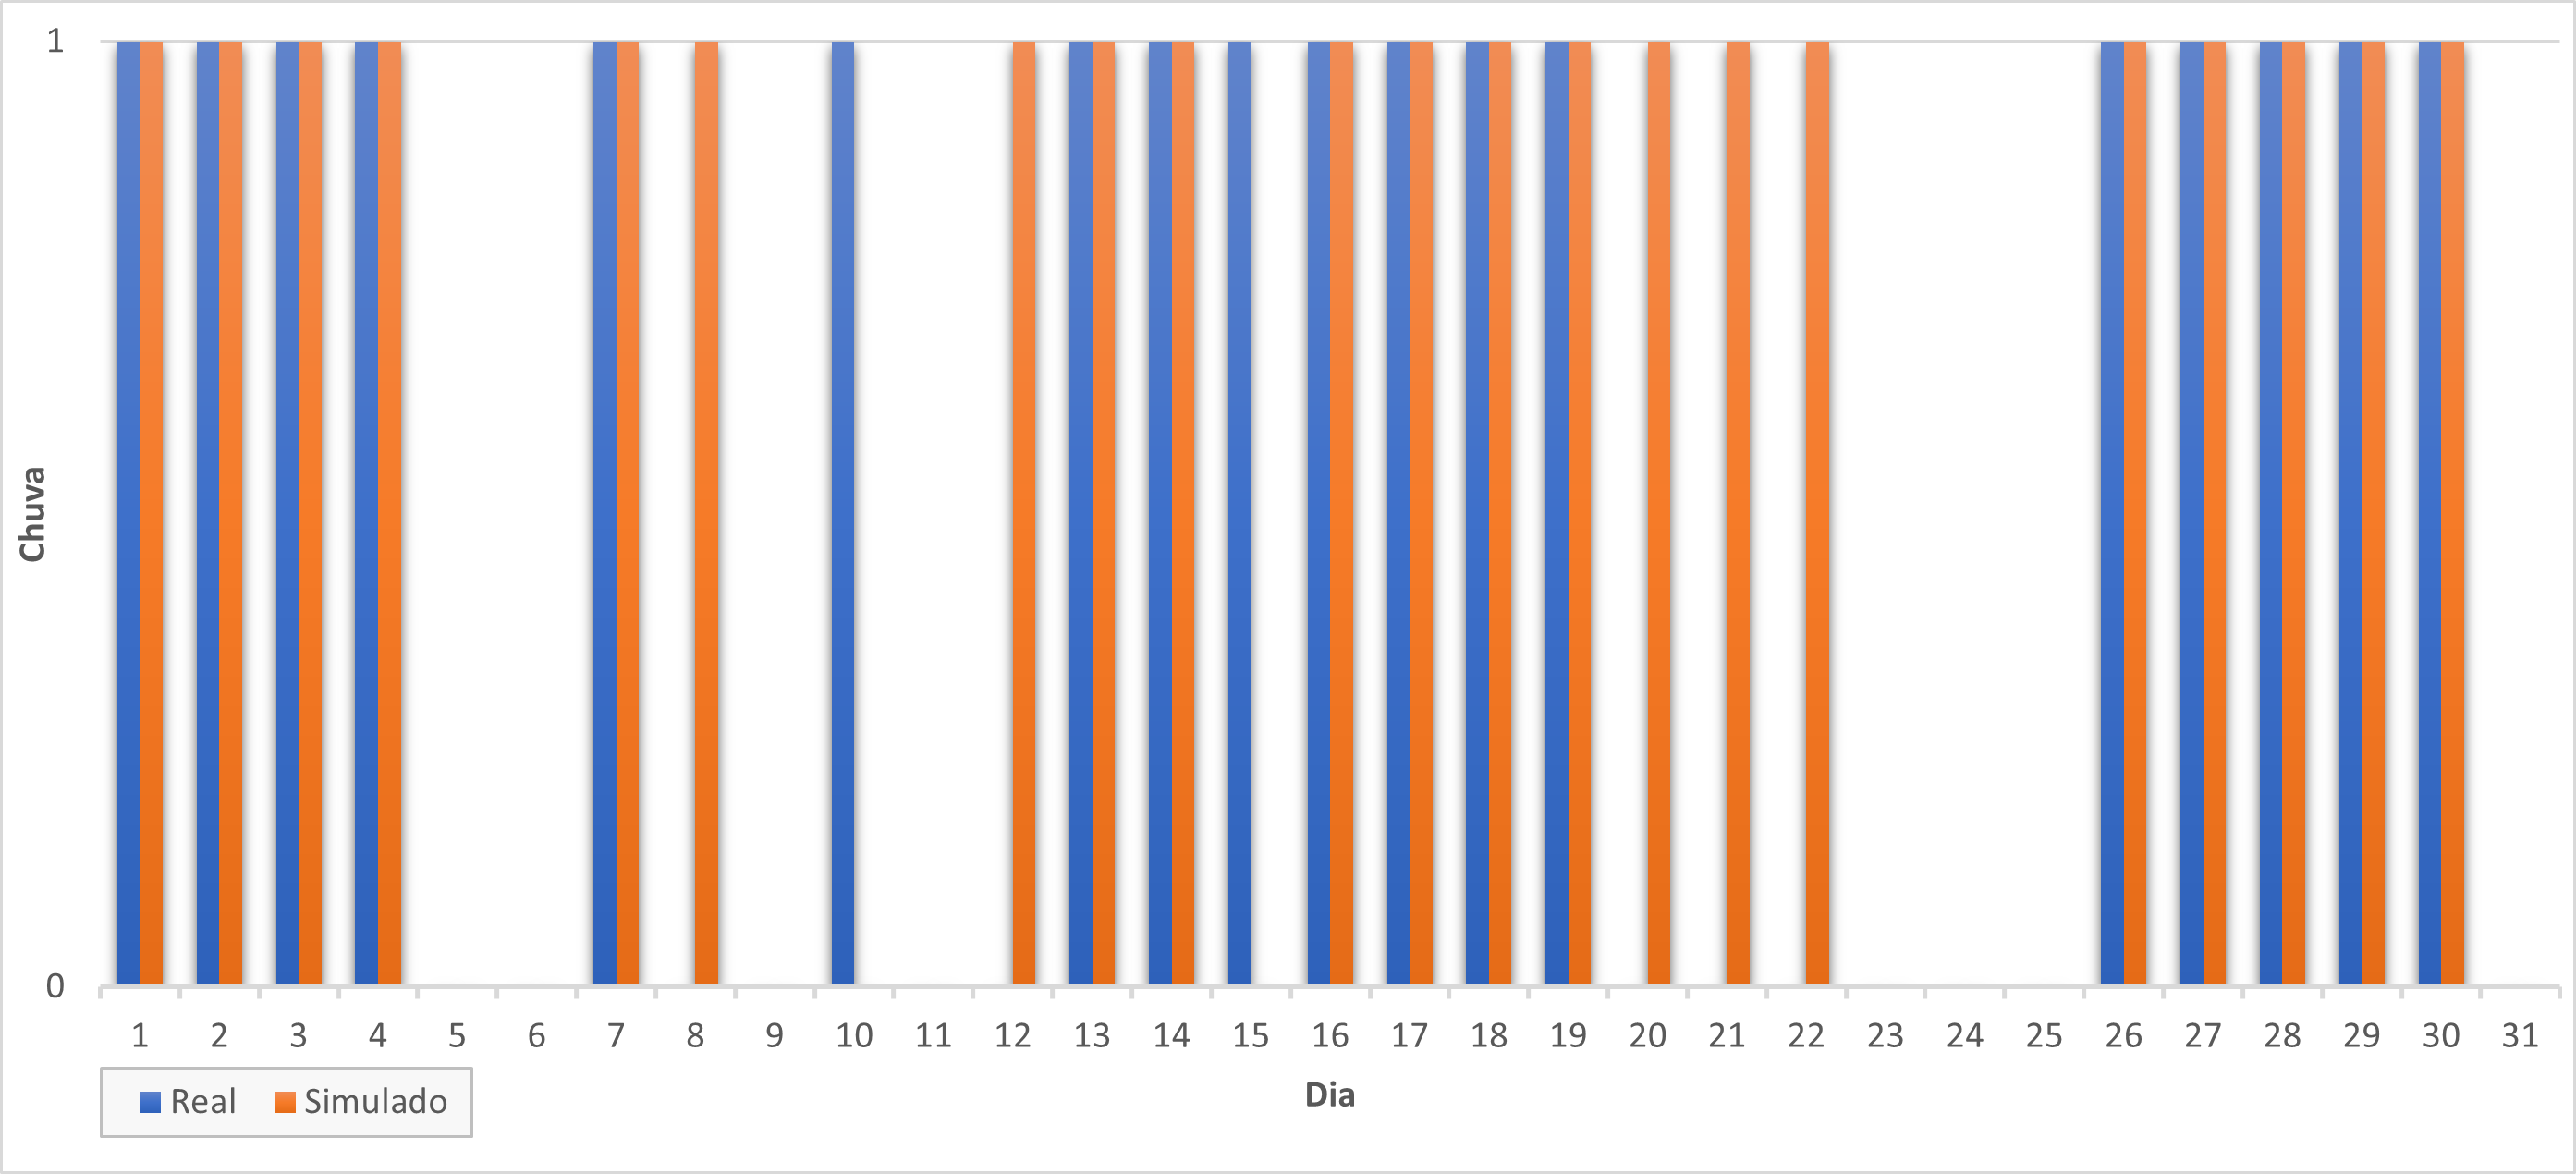
\includegraphics[width=\textwidth]{figs/jan.png}
	\label{f.rjan}
	\legend{\small Fonte: Elaborado pelo autor.}
\end{figure}

\subsection{Fevereiro}
Diferentemente de janeiro, a precisão para o mês de fevereiro não foi tão boa quanto. Uma das possíveis causas para isso são diversos fatores externos e imprevisíveis que podem ocorrer ocasionalmente. Ainda assim, com 15 erros e 13 acertos, a simulação previu corretamente 46,43\% dos dias de fevereiro.
\begin{figure}[H]
	\caption{\small Chuva x Dia - Fevereiro/2021}
	\centering
	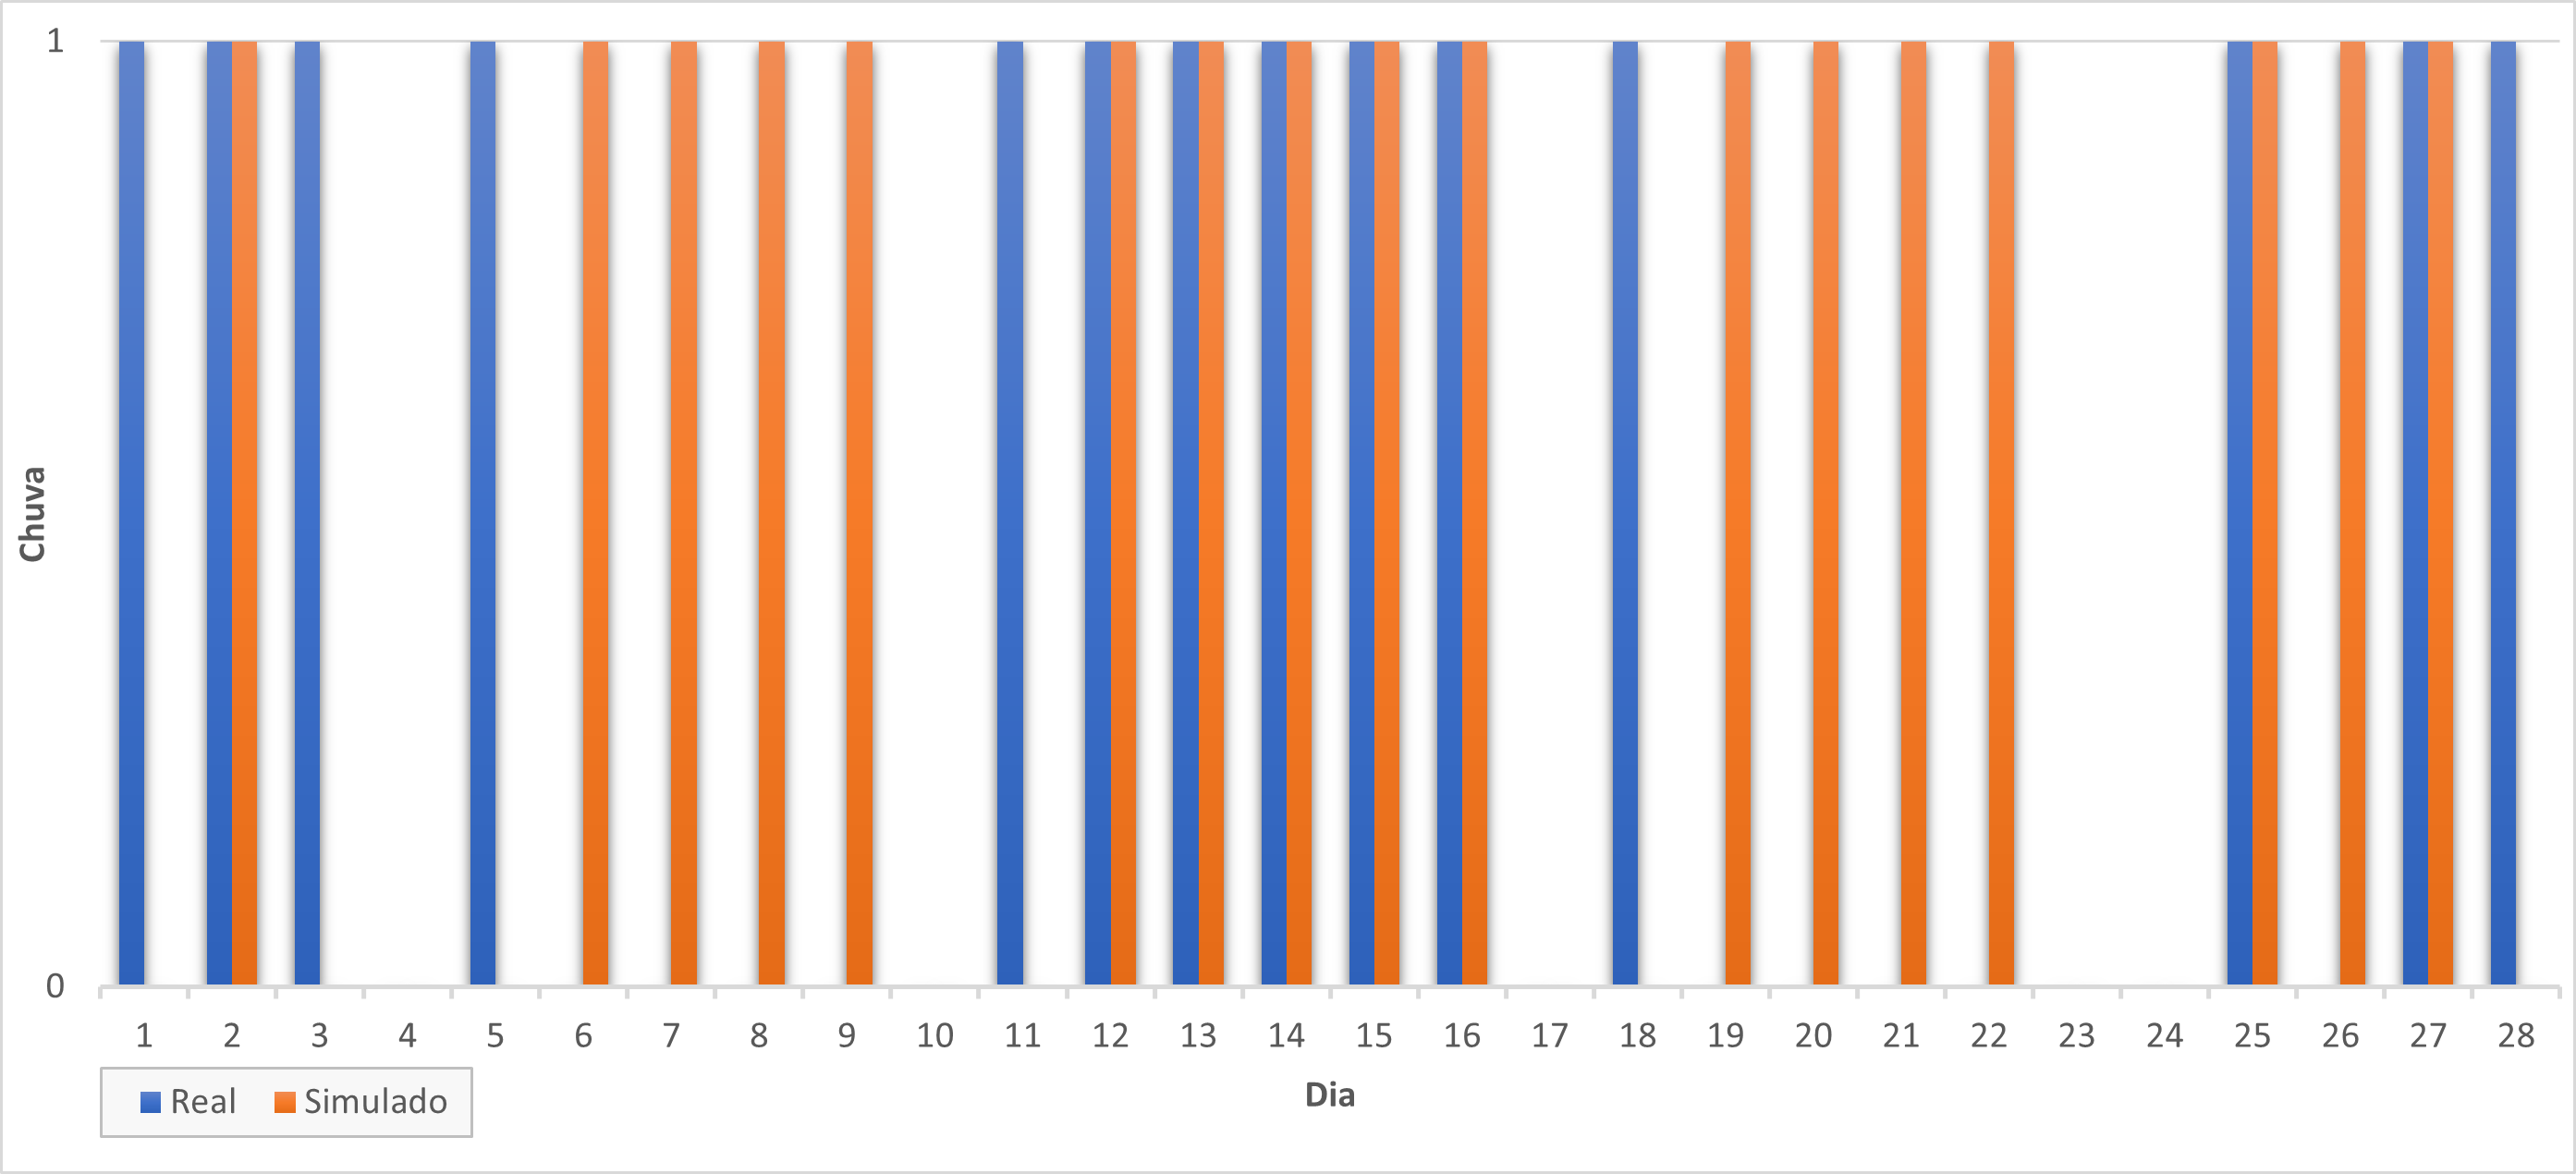
\includegraphics[width=\textwidth]{figs/fev.png}
	\label{f.rfev}
	\legend{\small Fonte: Elaborado pelo autor.}
\end{figure}

\subsection{Março}
Para o mês de março, apesar da simulação não ter tido um bom desempenho acerca dos dias que choveram, a previsão para os dias secos foi muito boa. Dos 21 dias que foram secos, 17 foram previstos corretamente, uma precisão de quase 81\% para os dias secos. No total dos dias de março, a precisão foi um pouco mais baixa, com 54,84\% de acerto.
\begin{figure}[H]
	\caption{\small Chuva x Dia - Março/2021}
	\centering
	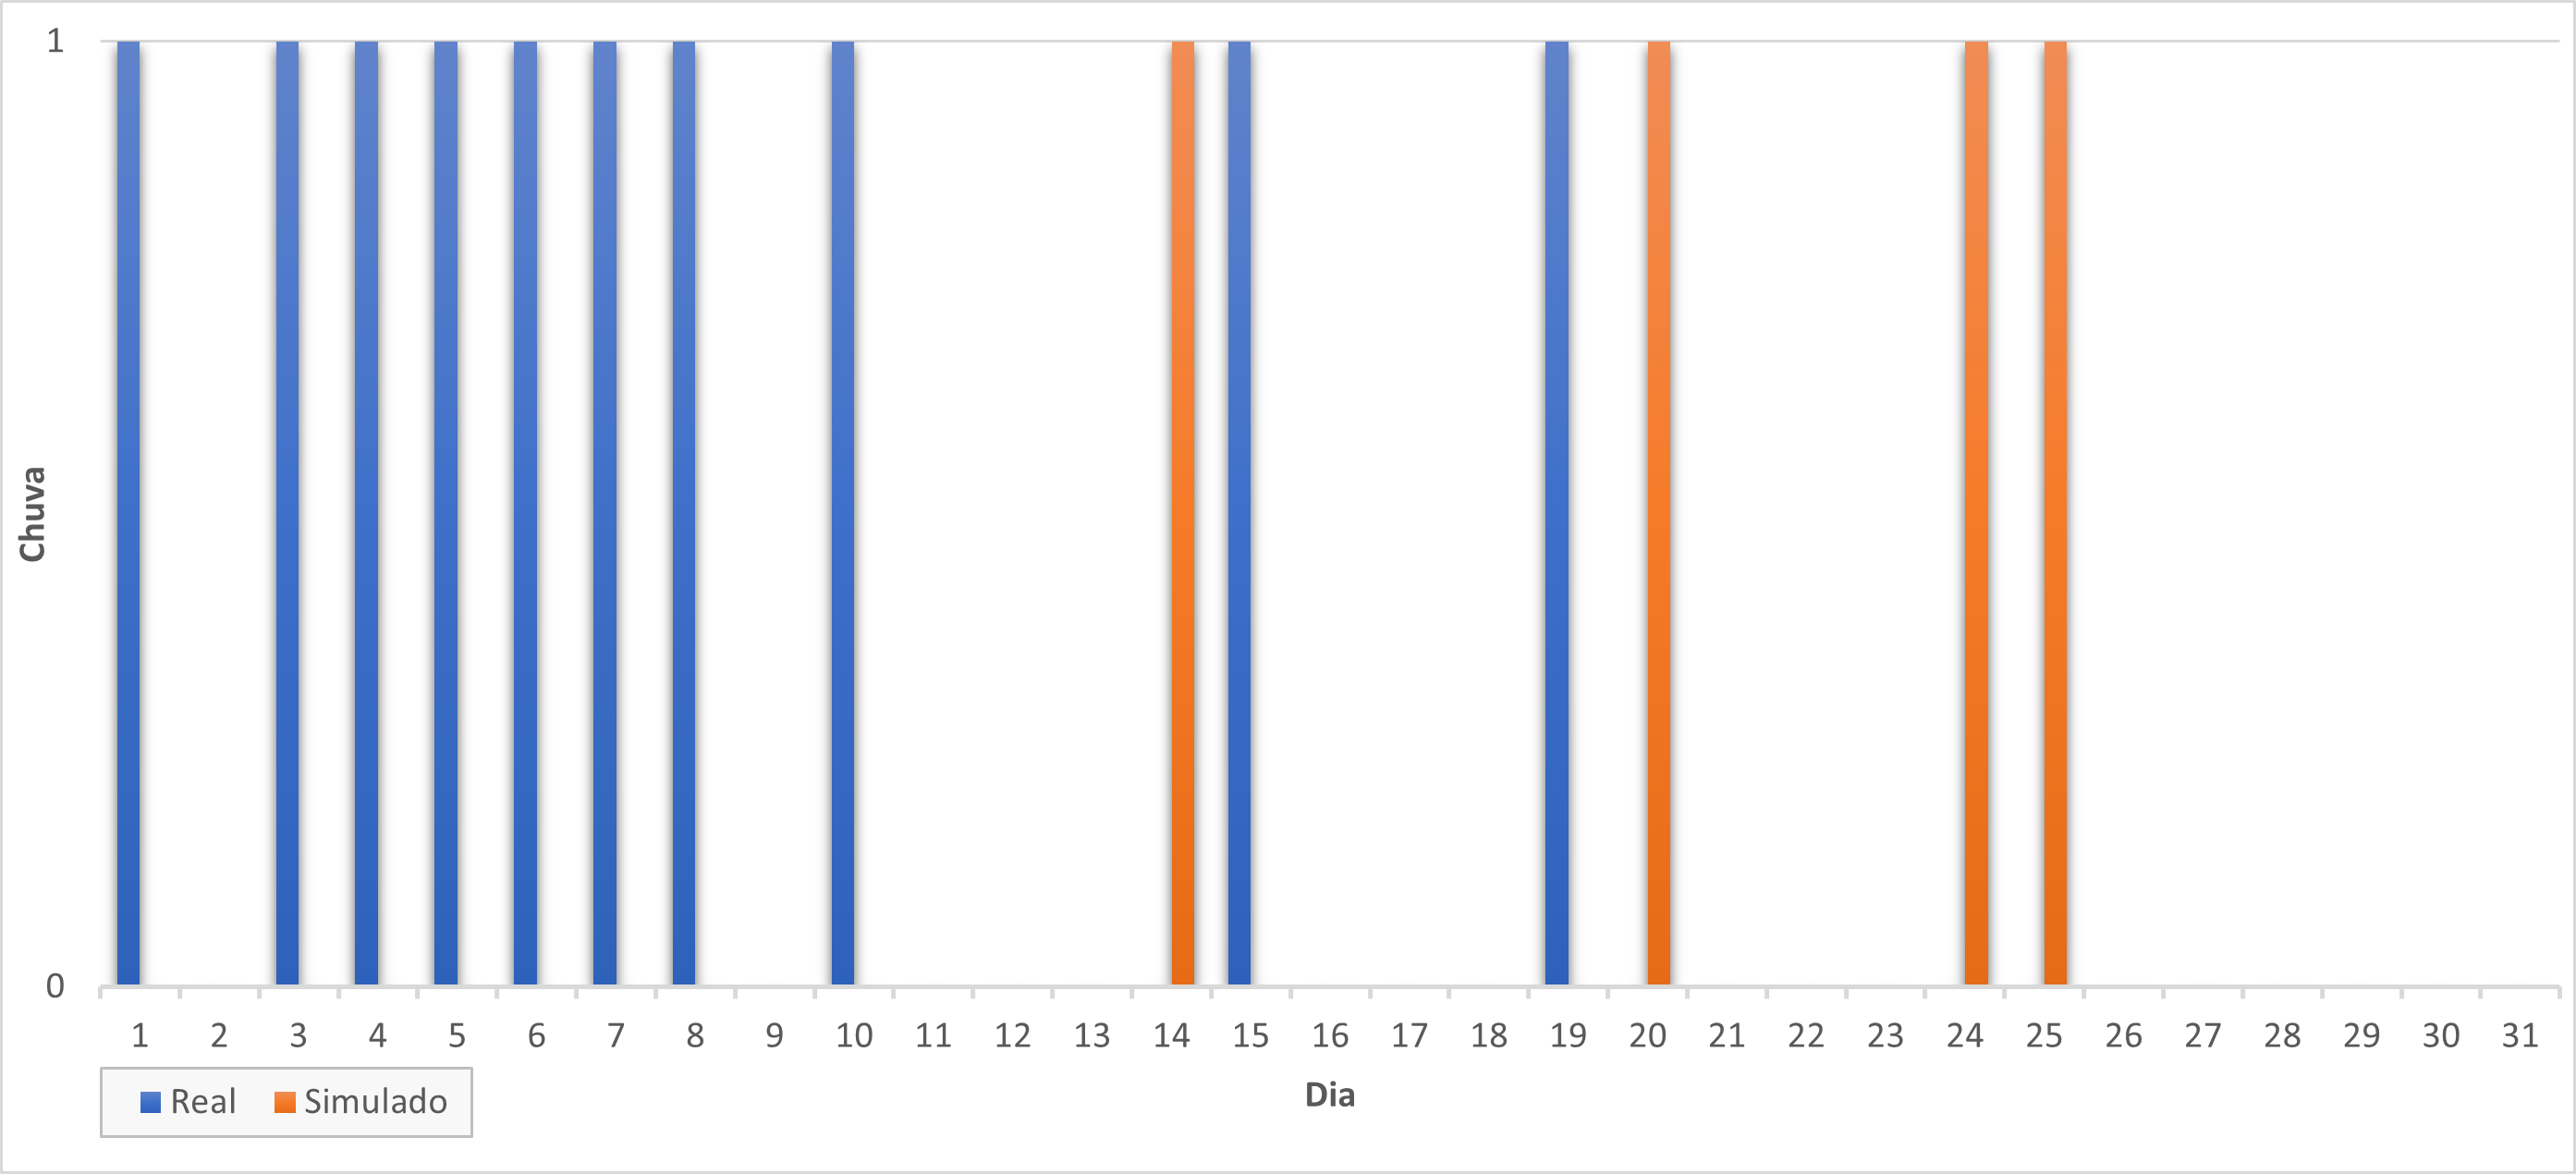
\includegraphics[width=\textwidth]{figs/mar.png}
	\label{f.rmar}
	\legend{\small Fonte: Elaborado pelo autor.}
\end{figure}

\subsection{Abril}
Com o fim da estação mais chuvosa da cidade, o grau de precisão também parece ser afetado um pouco. No mês de abril foram 19 acertos de 30 dias totais, uma taxa de 63,33\% de precisão da simulação computacional.
\begin{figure}[H]
	\caption{\small Chuva x Dia - Abril/2021}
	\centering
	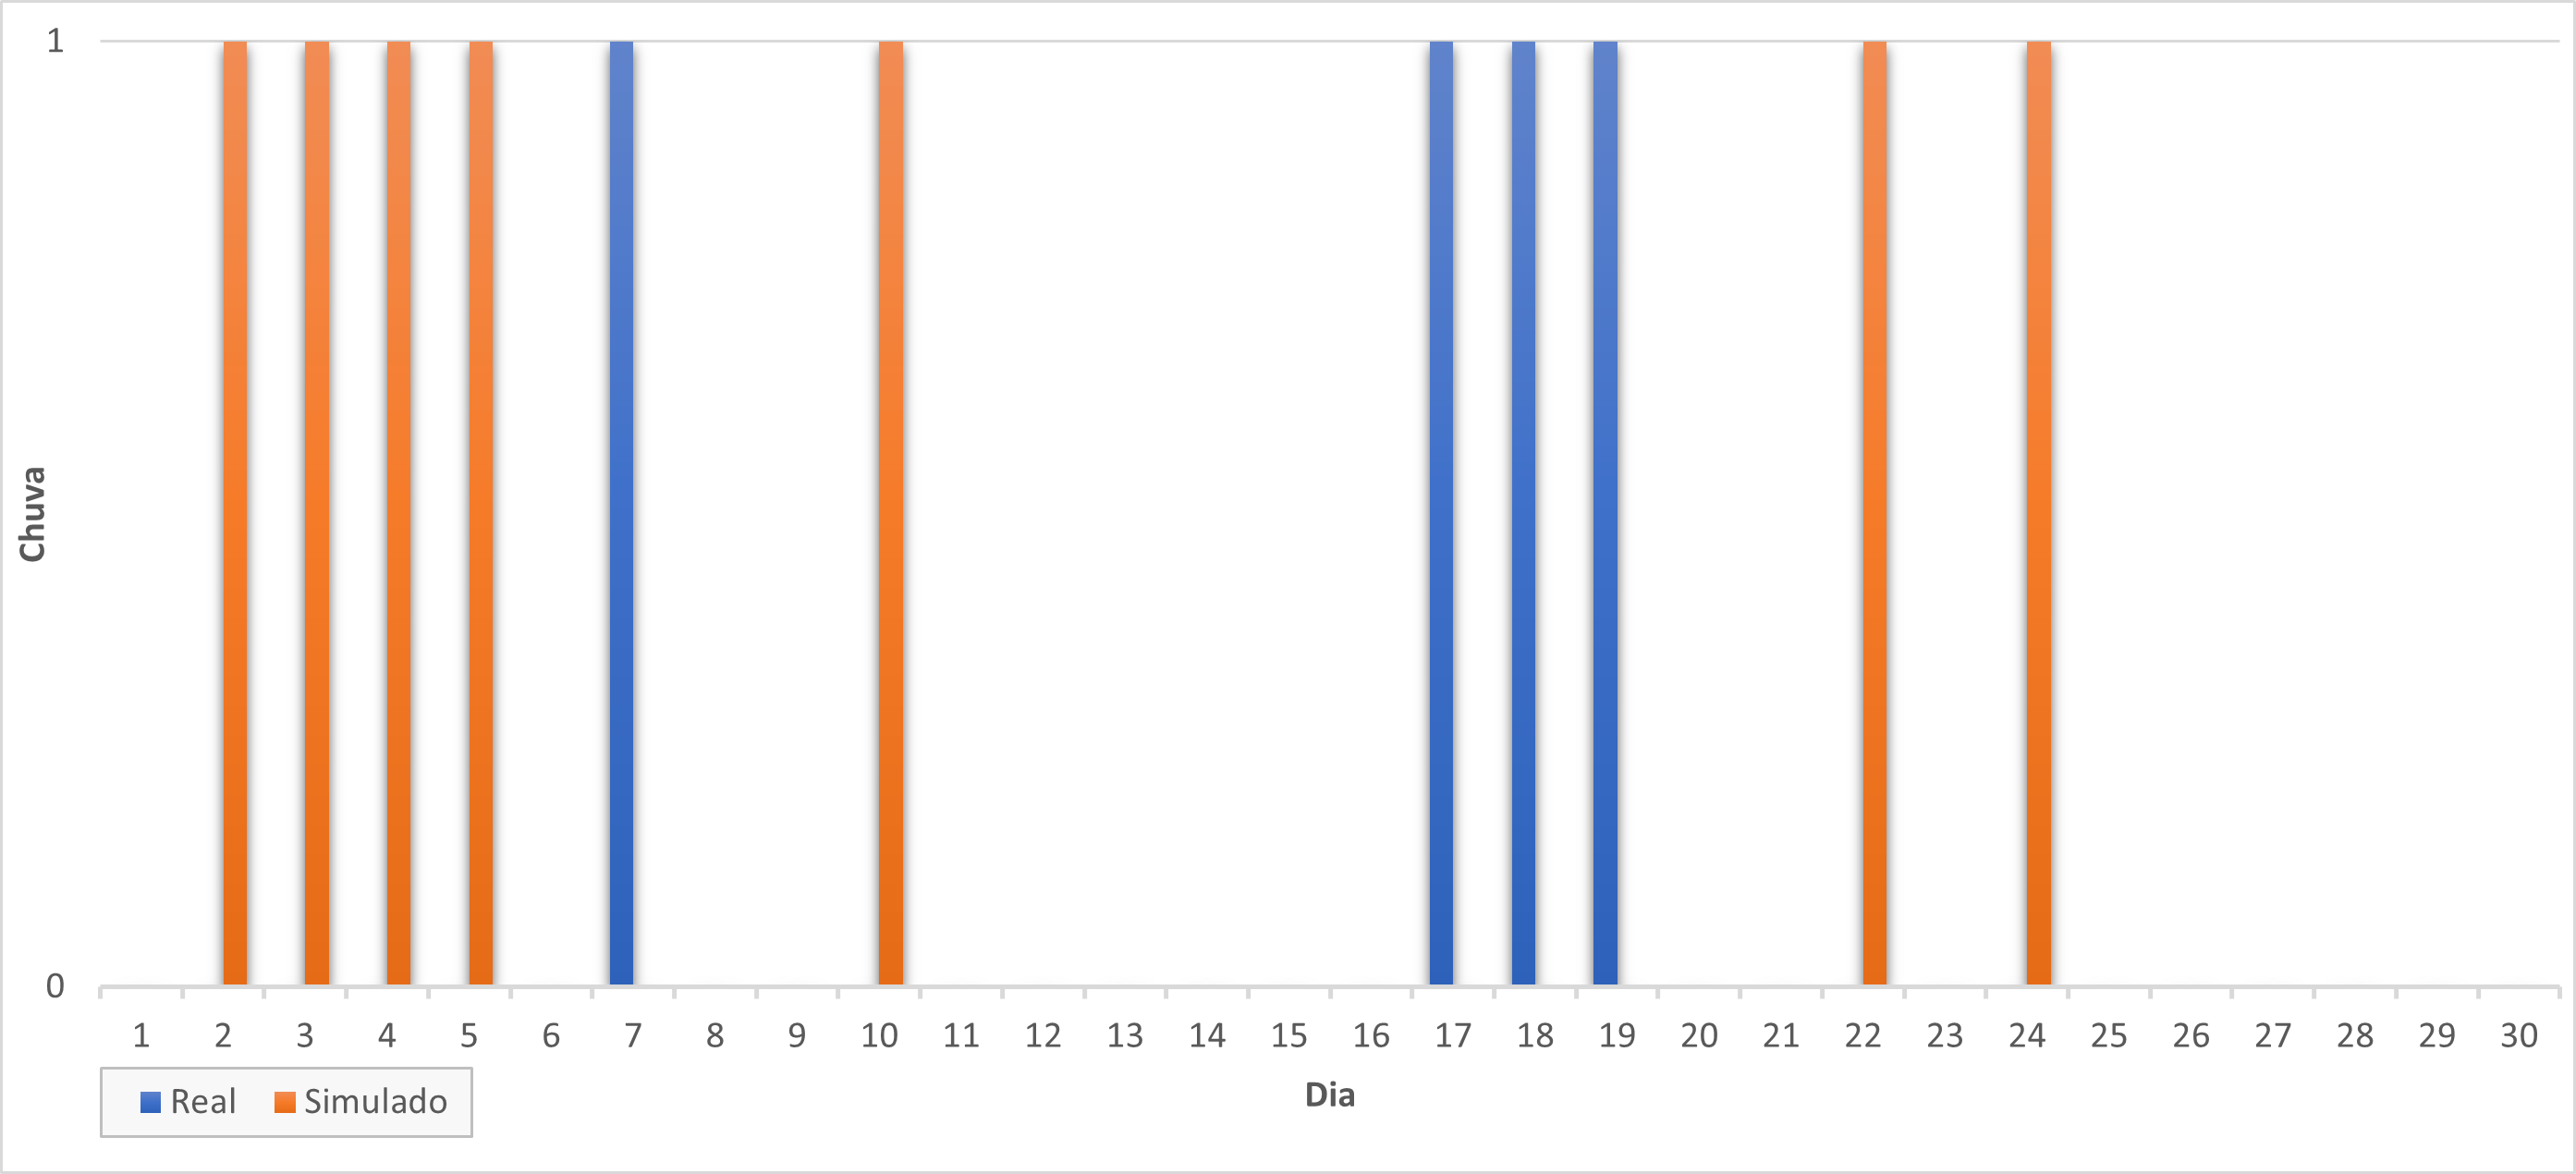
\includegraphics[width=\textwidth]{figs/abr.png}
	\label{f.rabr}
	\legend{\small Fonte: Elaborado pelo autor.}
\end{figure}

\subsection{Maio}
Em maio, apesar da simulação prever 10 dias chuvosos, por fatores externos houve apenas um dia chuvoso. No entanto, a maioria dos dias secos previstos foram certos. Portanto, a taxa de acerto, em geral, foi de 64,52\%, um resultado satisfatório dadas as circunstâncias de um mês atípico.
\begin{figure}[H]
	\caption{\small Chuva x Dia - Maio/2021}
	\centering
	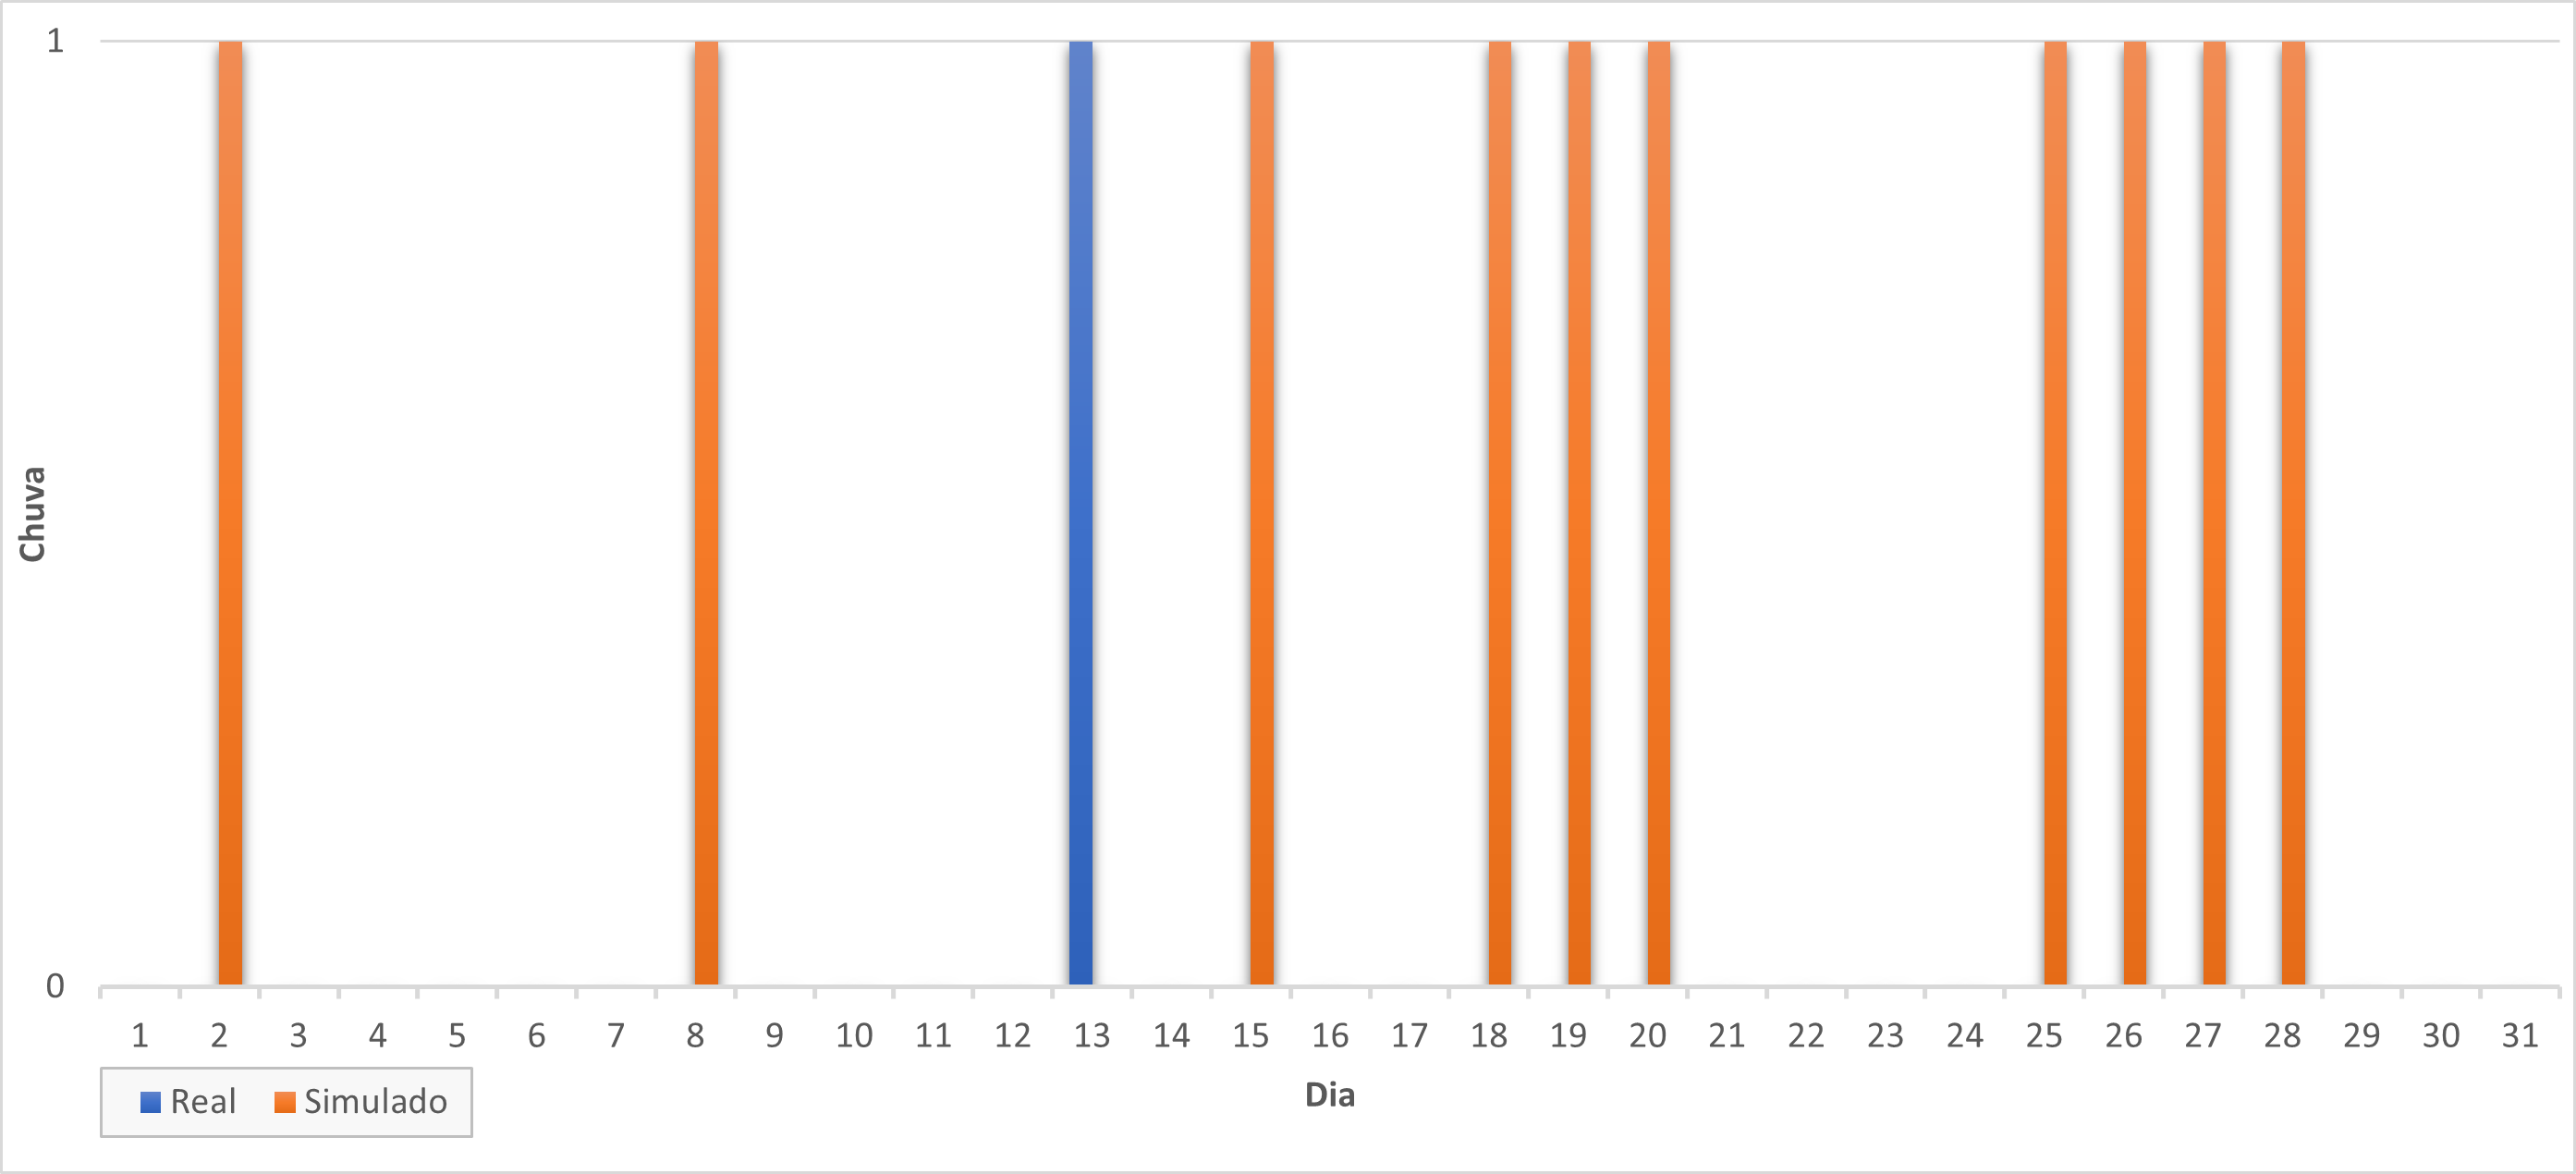
\includegraphics[width=\textwidth]{figs/mai.png}
	\label{f.rmai}
	\legend{\small Fonte: Elaborado pelo autor.}
\end{figure}

\subsection{Junho}
No meio do ano, em junho de 2021, foram 6 dias chuvosos no total. A simulação previu 4 dias chuvosos no mesmo mês, porém em dias diferentes. Em geral, com os acertos dos dias secos previstos, a chuva de 66,67\% dos dias foi simulada corretamente.
\begin{figure}[H]
	\caption{\small Chuva x Dia - Junho/2021}
	\centering
	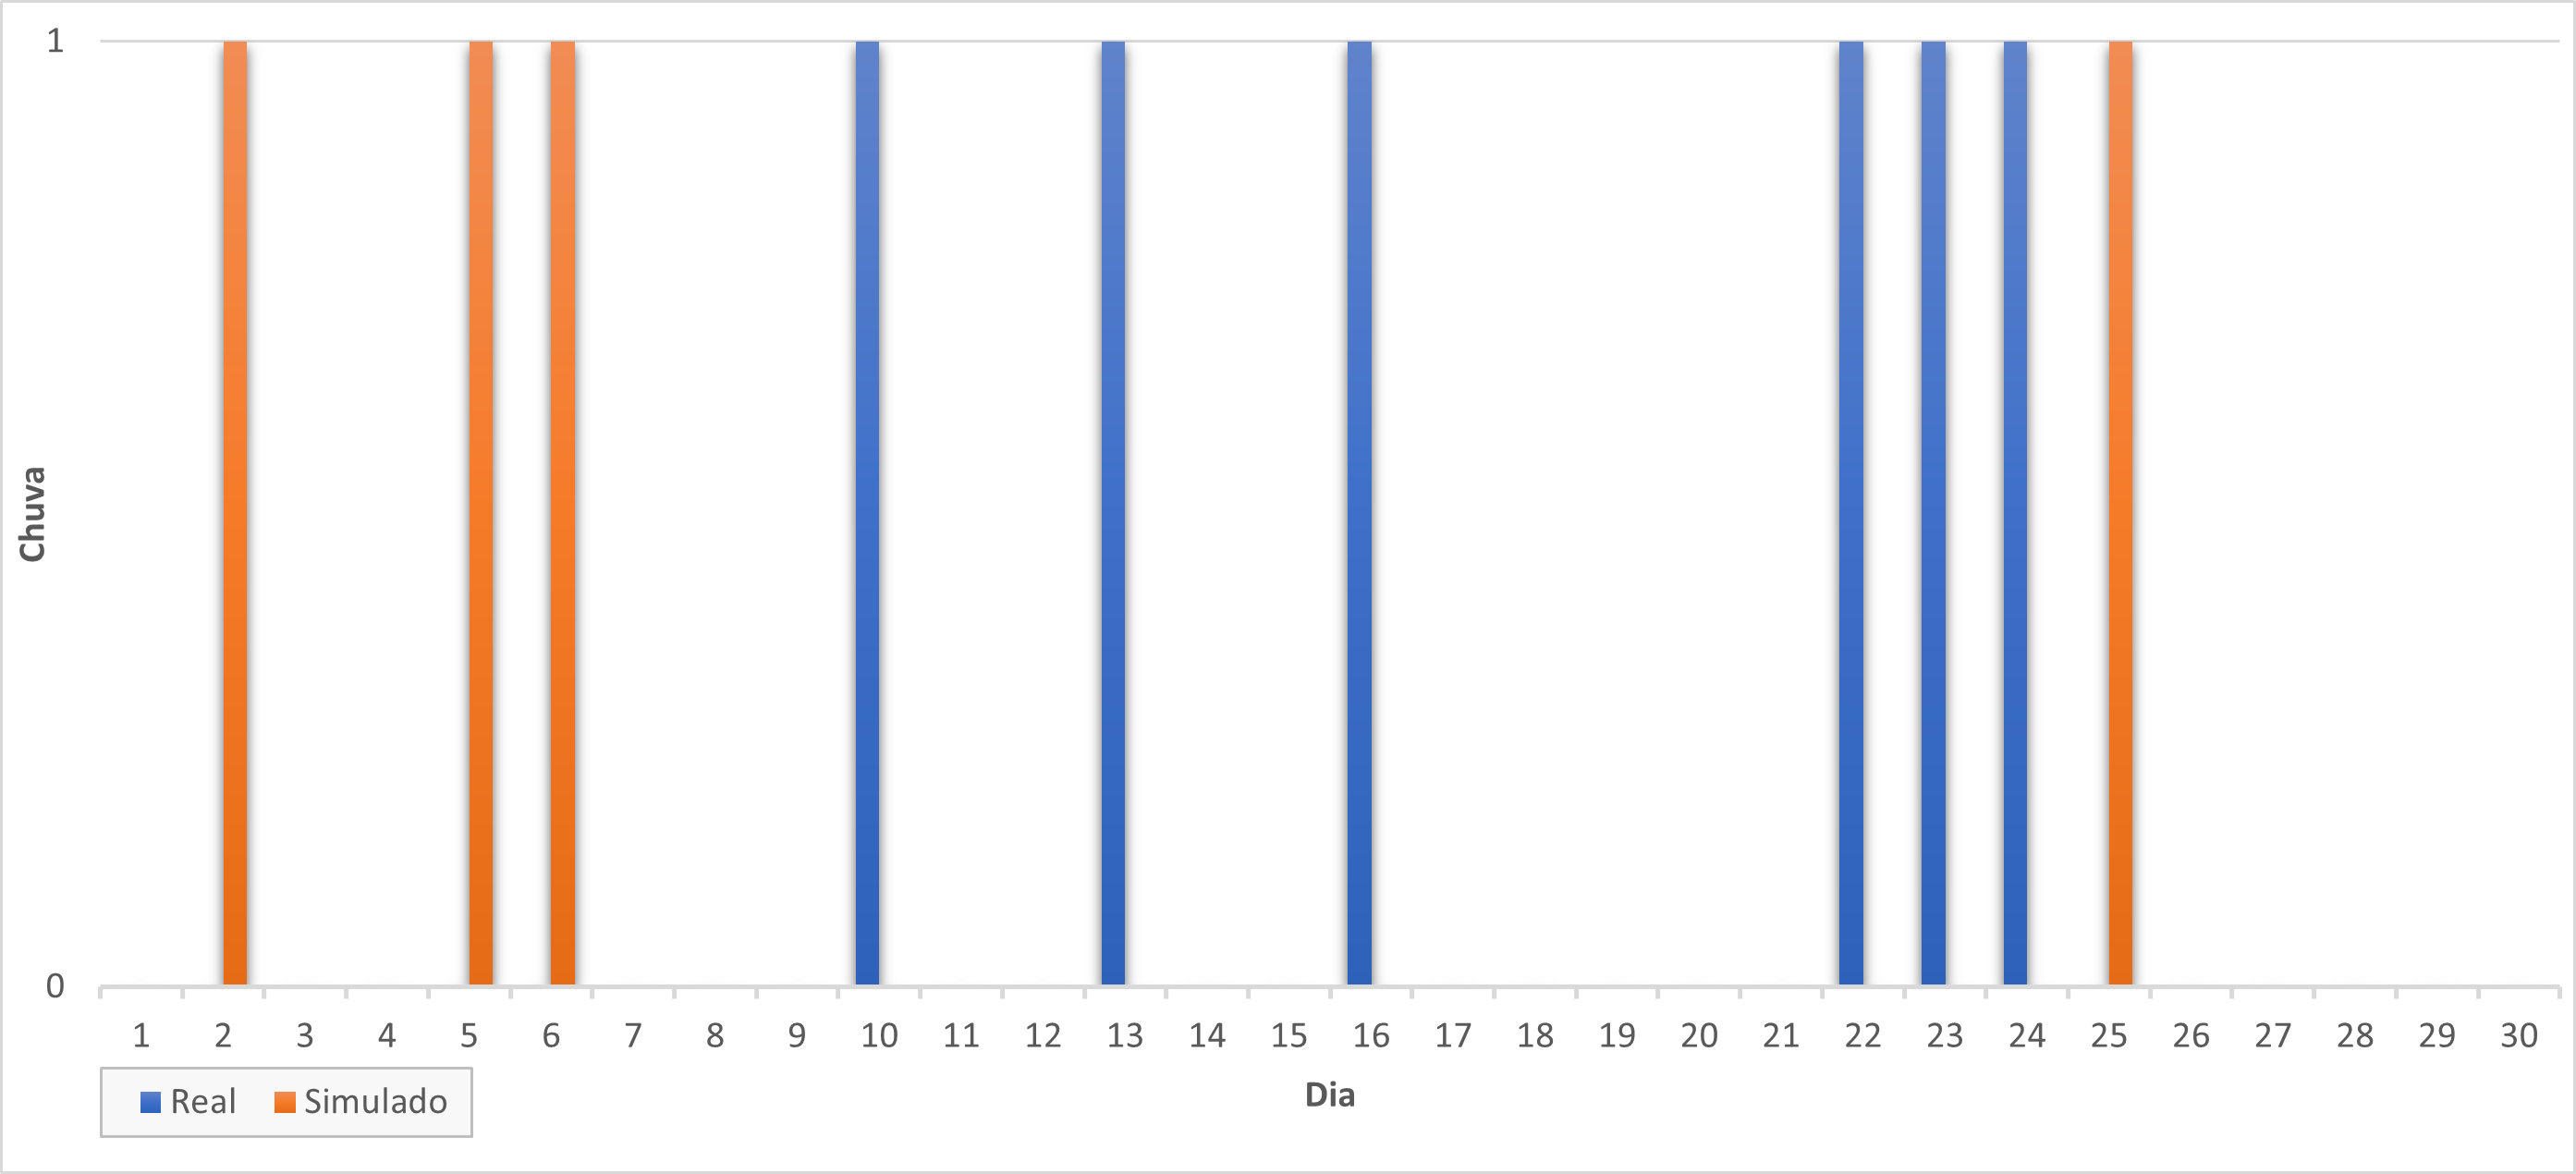
\includegraphics[width=\textwidth]{figs/jun.png}
	\label{f.rjun}
	\legend{\small Fonte: Elaborado pelo autor.}
\end{figure}

\subsection{Julho}
O meio do ano é a data mais seca da cidade de Bauru, com poucos dias de chuvas esporádicas na região. Assim, conforme observado no gráfico da figura \ref{f.rjul}, dos 31 dias de julho, 29 foram previstos corretamente, com uma taxa de acerto de 93,55\%.
\begin{figure}[H]
	\caption{\small Chuva x Dia - Julho/2021}
	\centering
	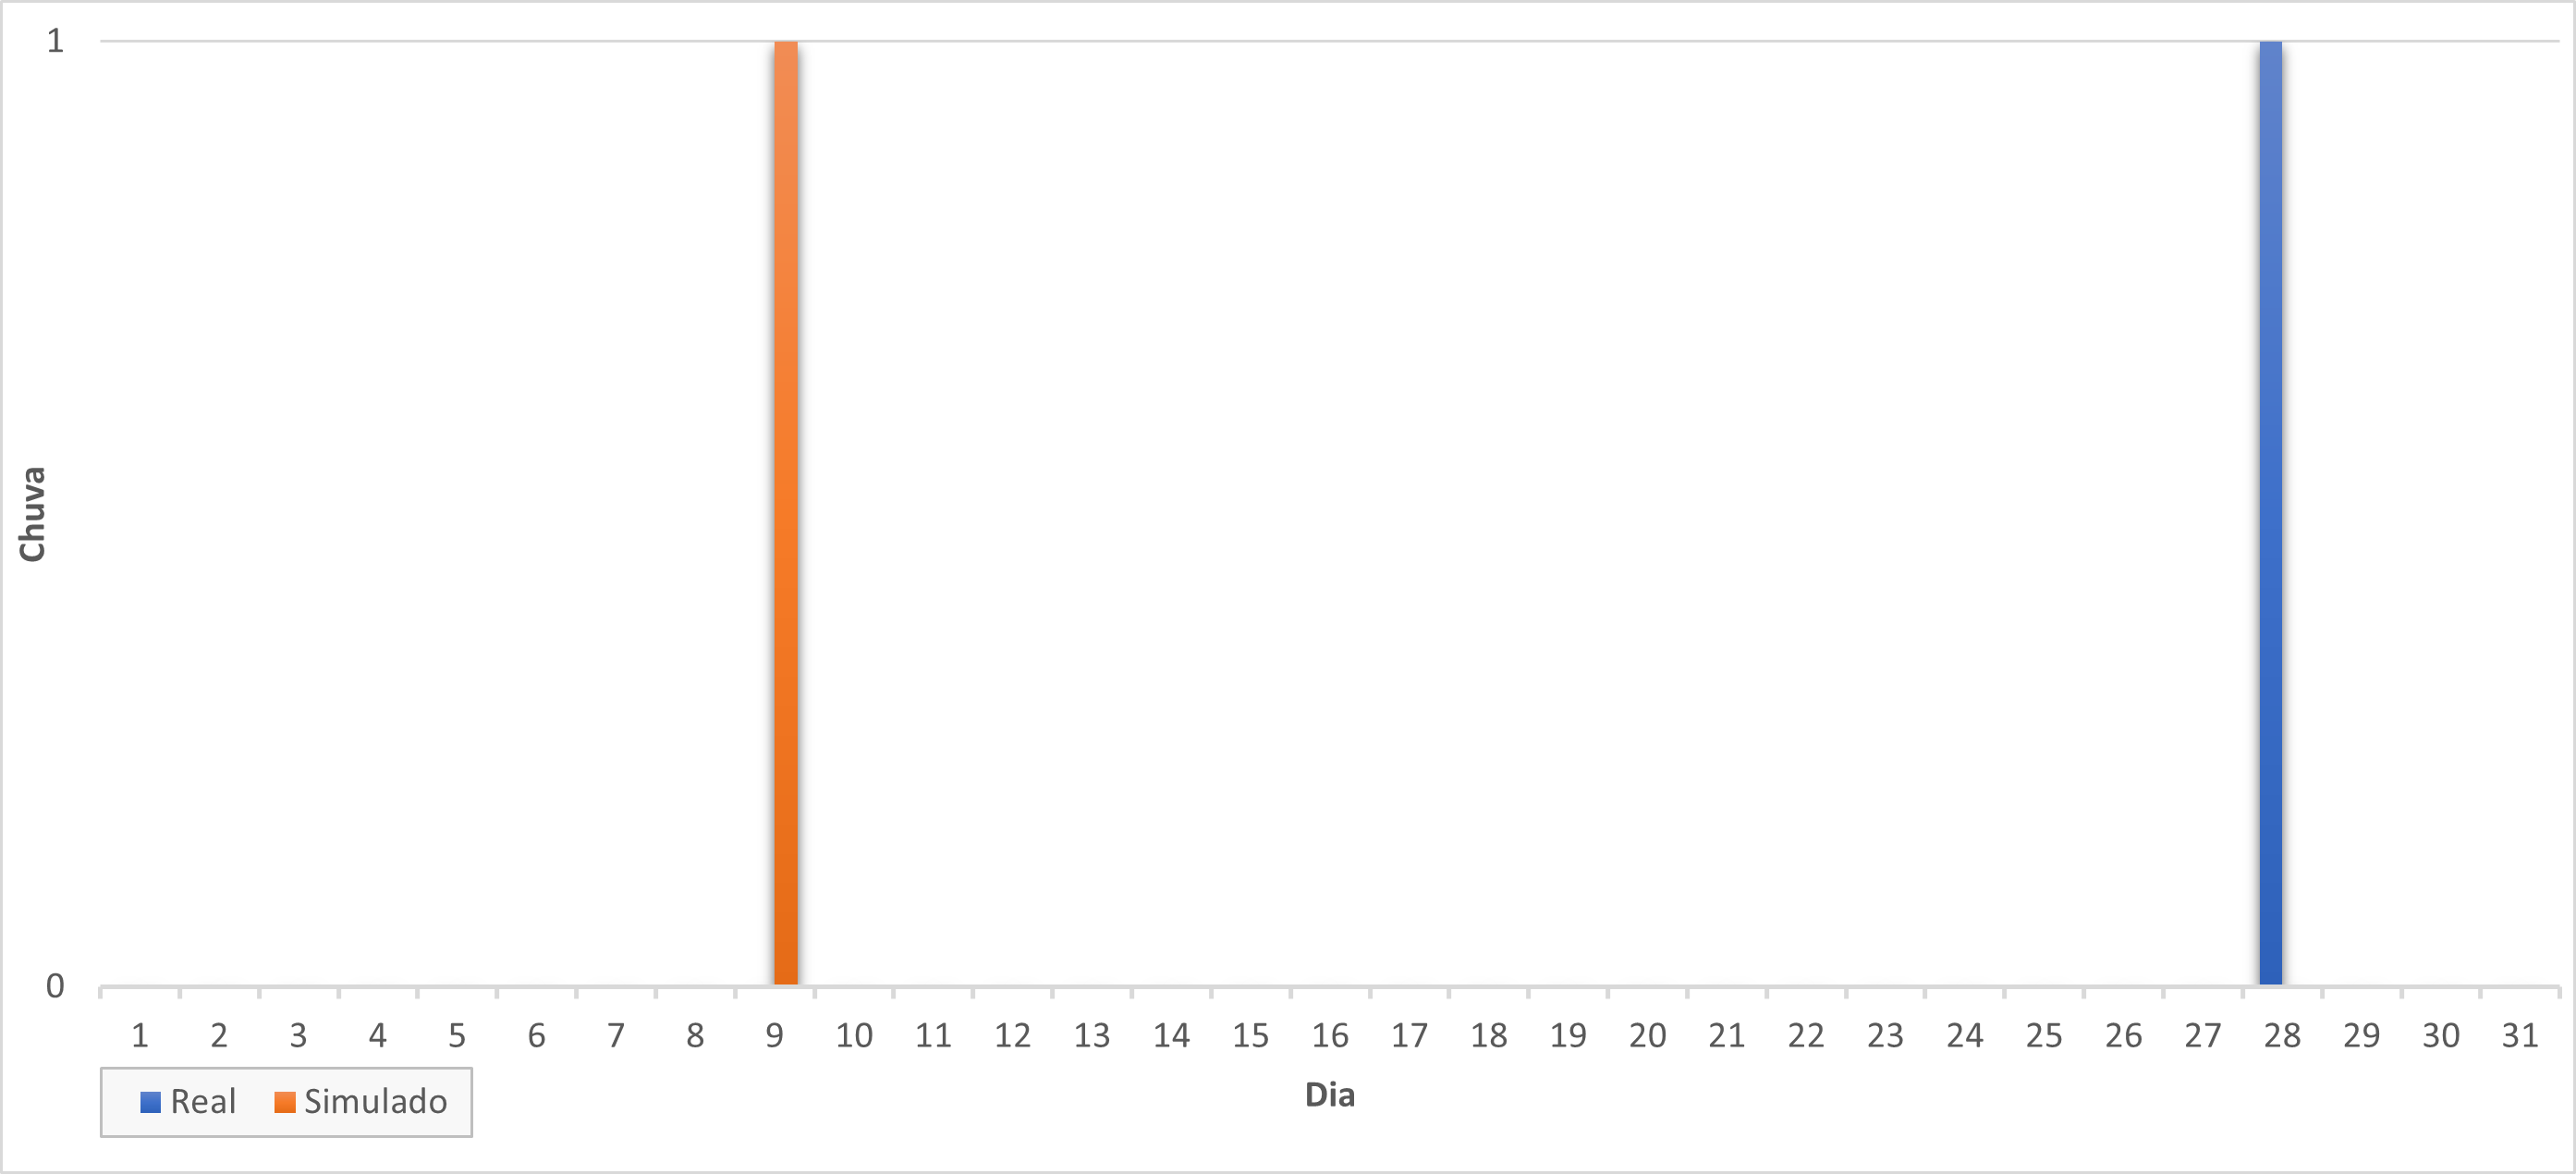
\includegraphics[width=\textwidth]{figs/jul.png}
	\label{f.rjul}
	\legend{\small Fonte: Elaborado pelo autor.}
\end{figure}

\subsection{Agosto}
O mesmo ocorreu em agosto, que na realidade, por algum motivo, choveu 2 dias consecutivos enquanto a simulação previu que todos os 31 dias seriam secos. A taxa de acerto foi a mesma do mês de julho, 93,55\%.
\begin{figure}[H]
	\caption{\small Chuva x Dia - Agosto/2021}
	\centering
	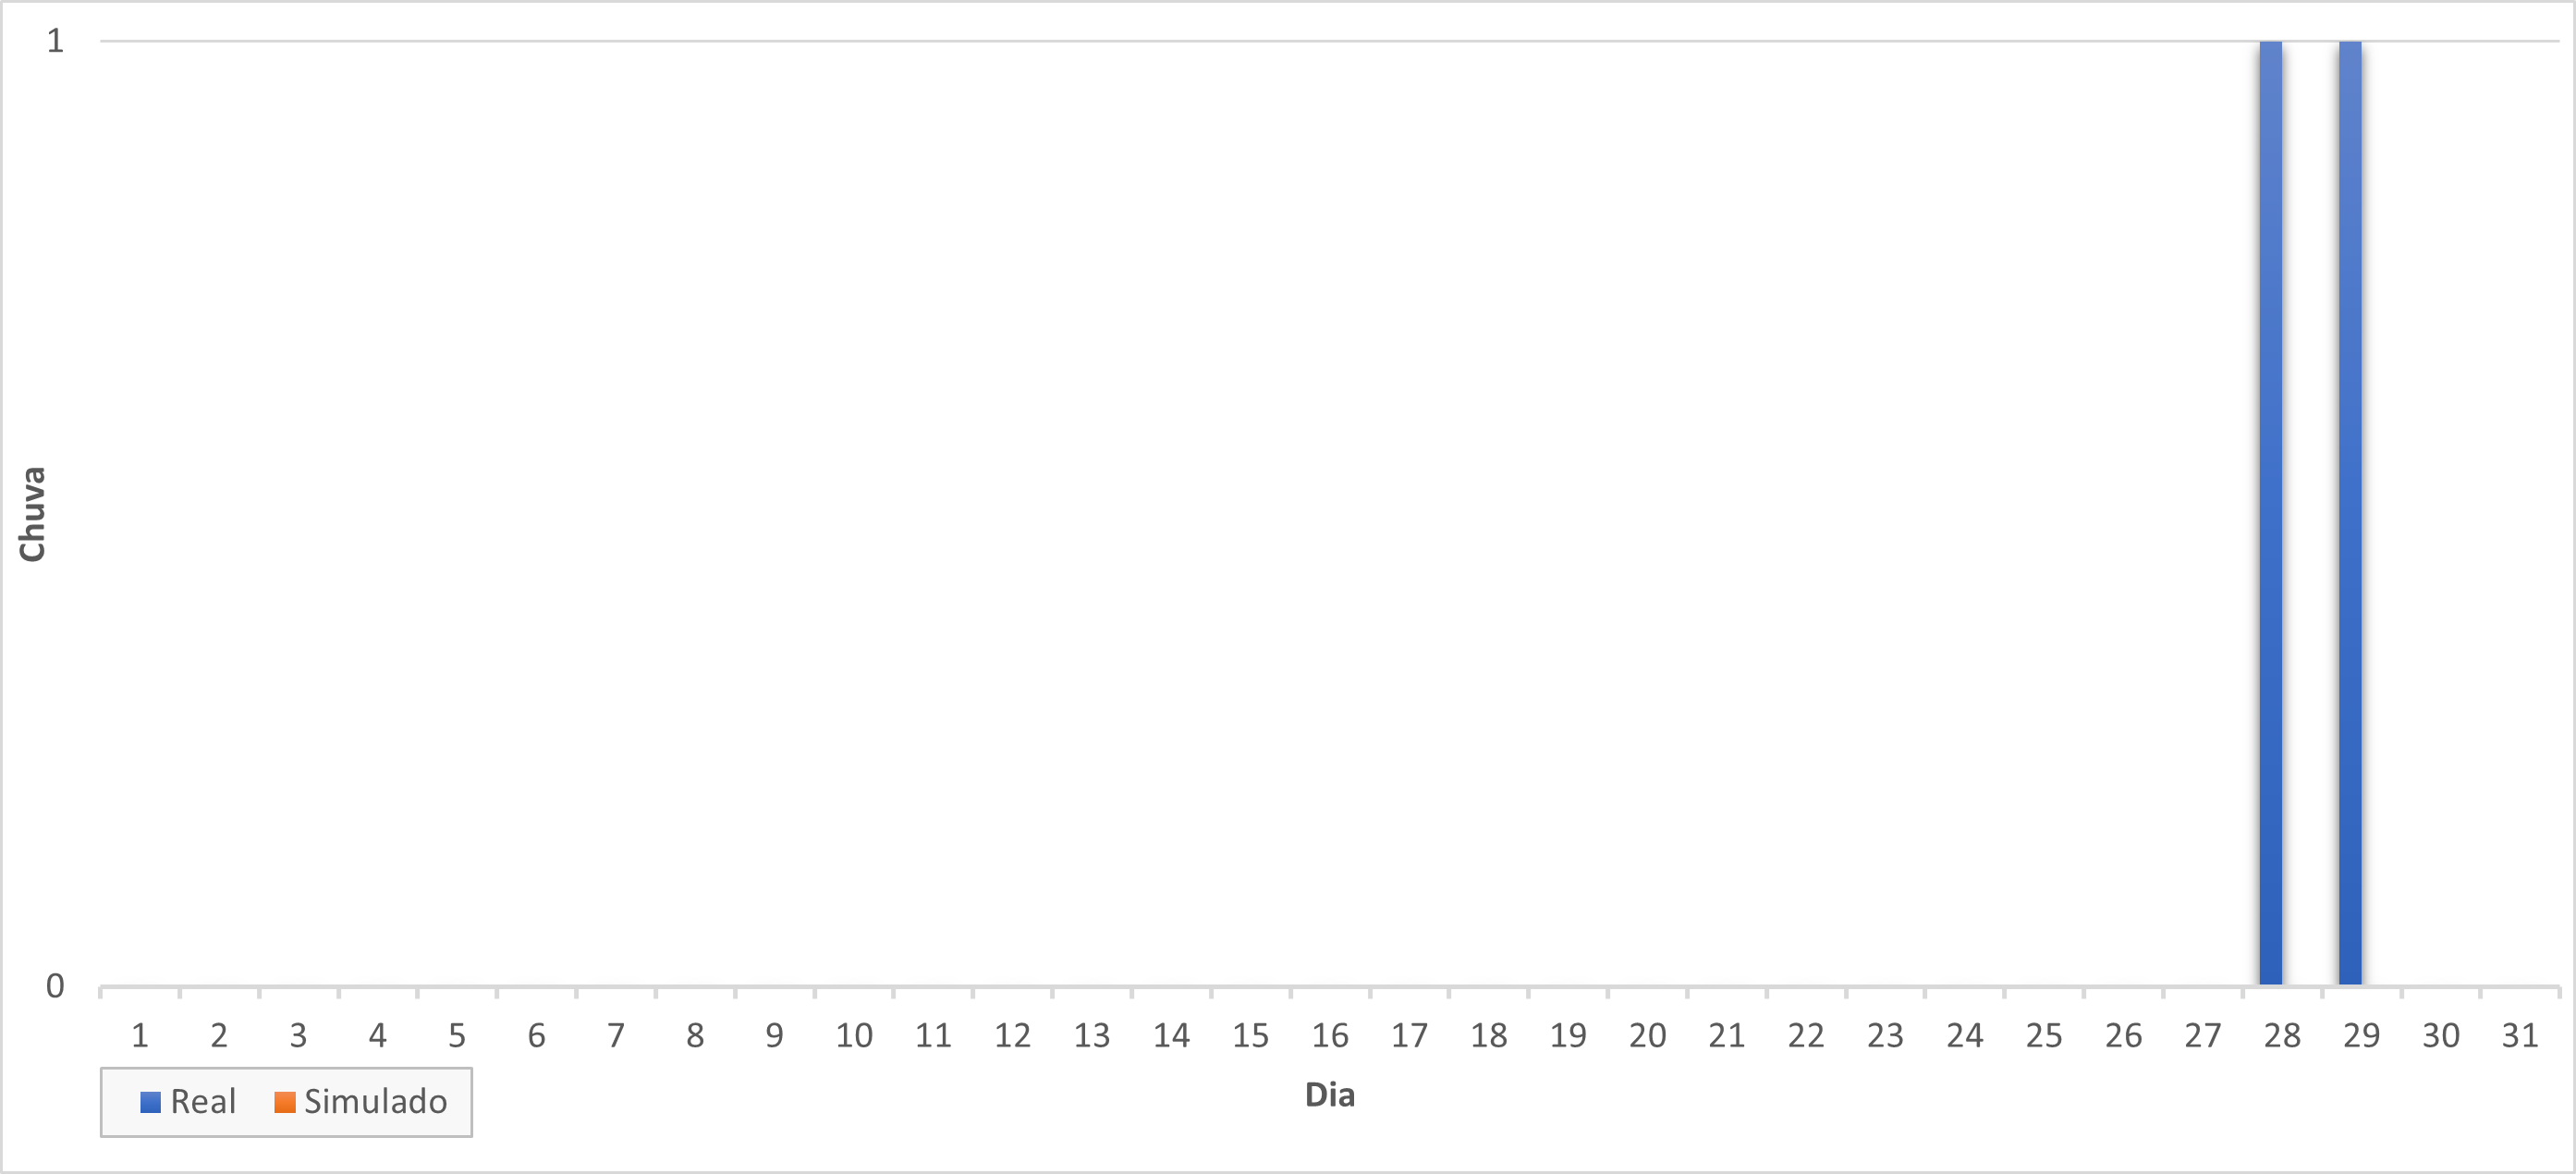
\includegraphics[width=\textwidth]{figs/ago.png}
	\label{f.rago}
	\legend{\small Fonte: Elaborado pelo autor.}
\end{figure}

\subsection{Setembro}
No mês de setembro, que tem 30 dias, a simulação errou apenas 5 dias. O destaque ficou a partir do dia 9, onde na figura \ref{f.rset} é possível notar que o início dos dias chuvosos do mês foi previsto de maneira exata. O resultado foi 83,33\% de acerto.
\begin{figure}[H]
	\caption{\small Chuva x Dia - Setembro/2021}
	\centering
	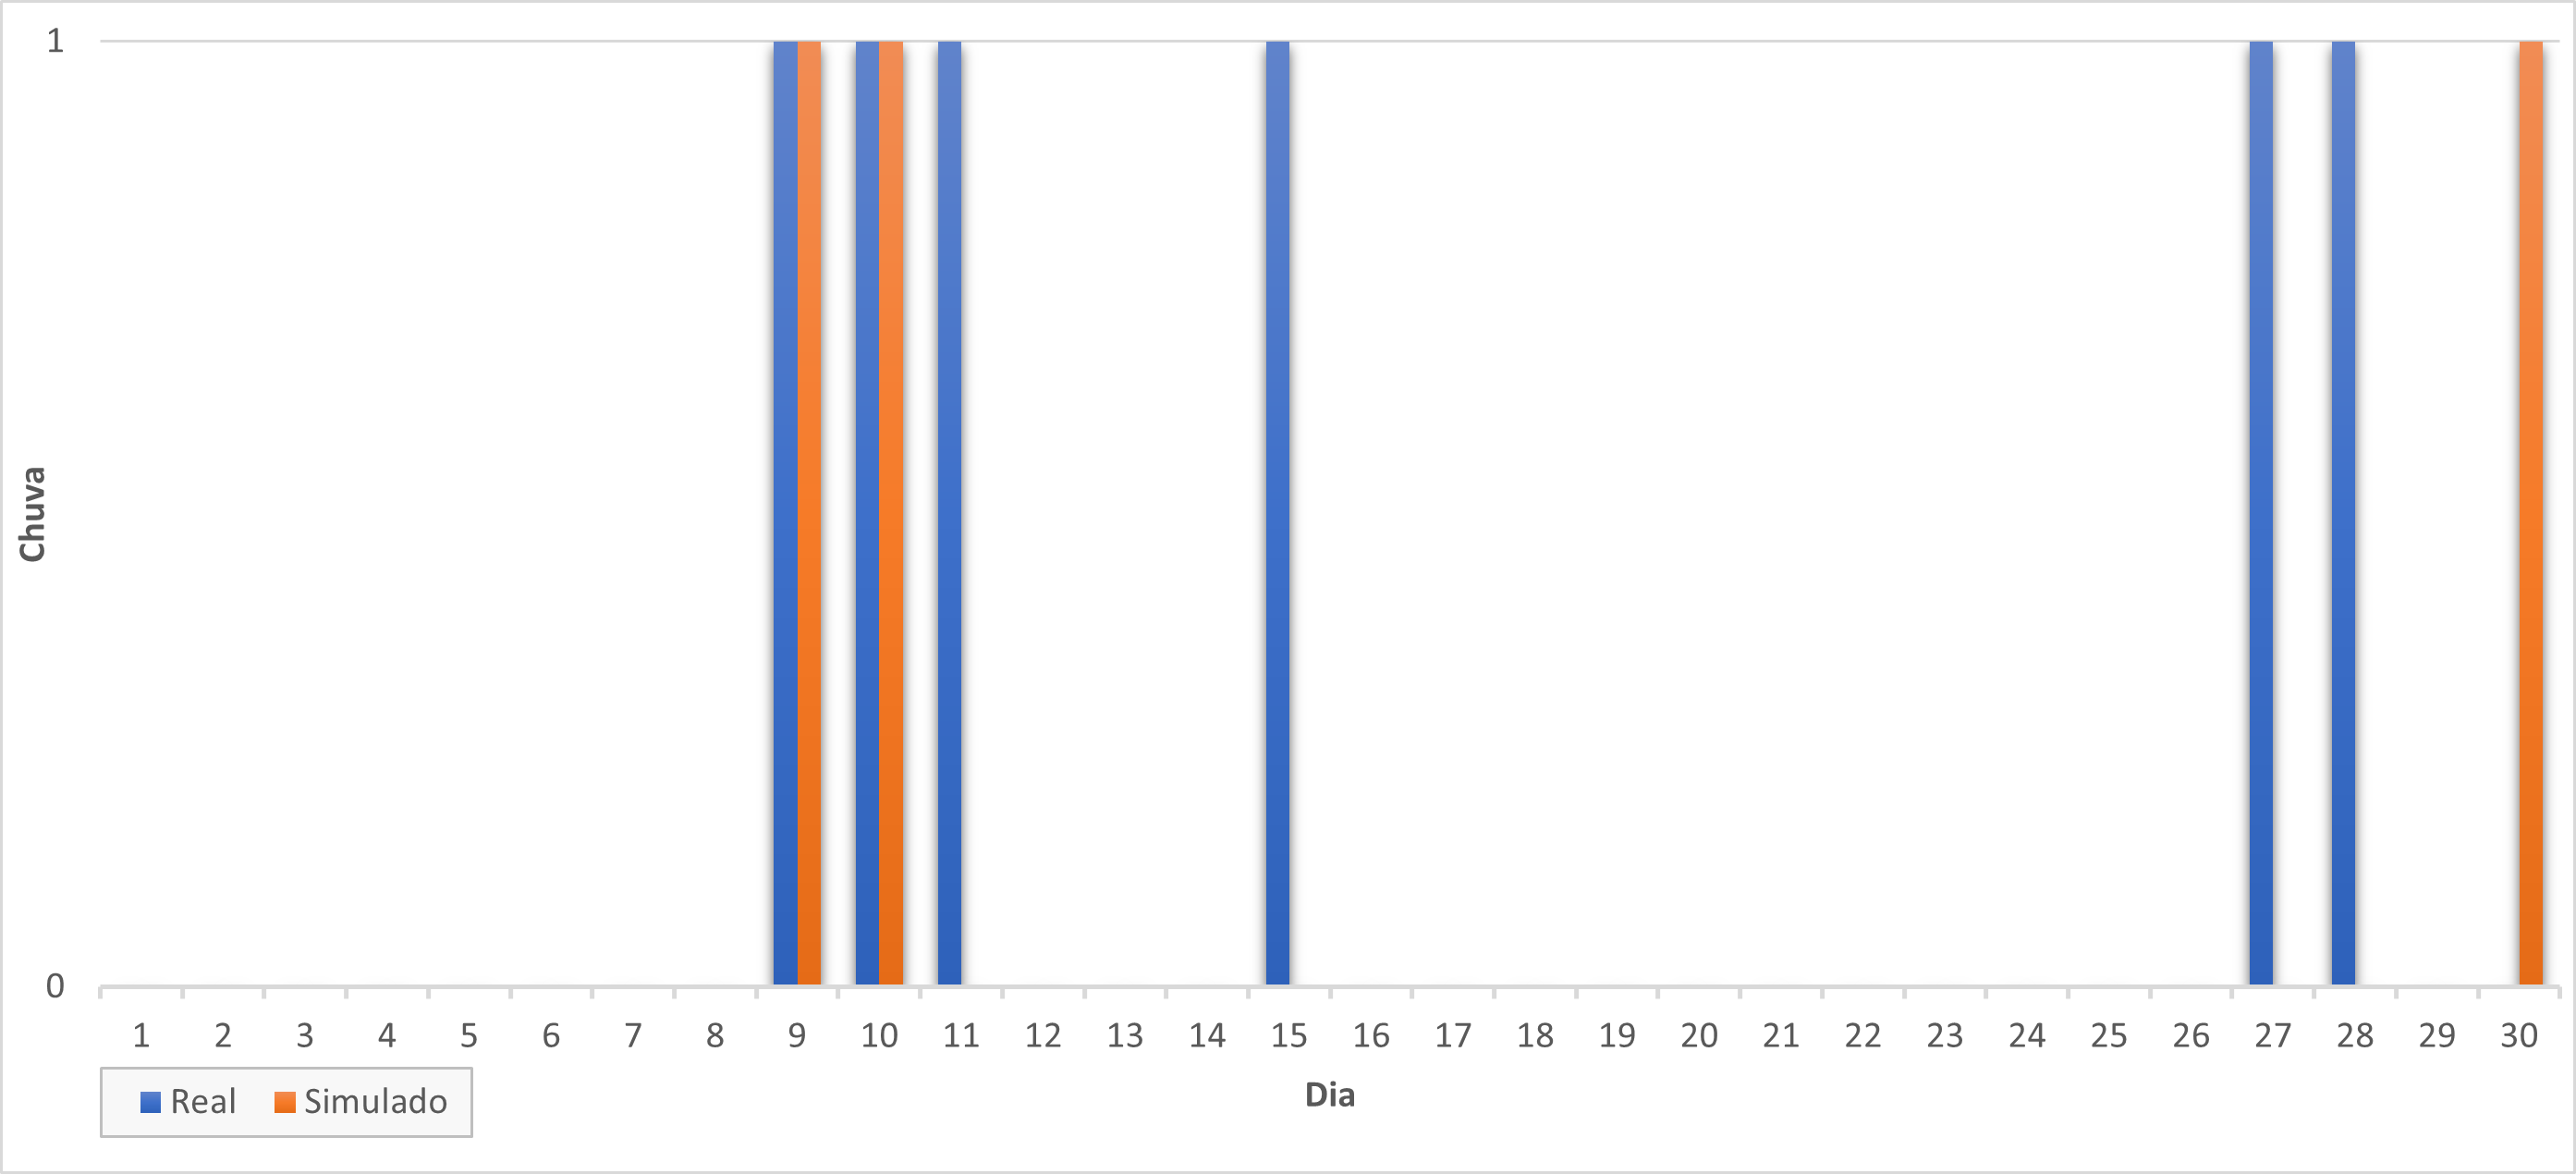
\includegraphics[width=\textwidth]{figs/set.png}
	\label{f.rset}
	\legend{\small Fonte: Elaborado pelo autor.}
\end{figure}

\subsection{Outubro}
Com a volta do verão, estação mais chuvosa da cidade, a expectativa é de que mais dias chuvosos apareçam no gráfico dos resultados. Assim sendo, na figura \ref{f.rout} é possível observar que outubro realmente foi bastante chuvoso, tanto nos dados reais, em cor azul, quanto nos dados simulados, em cor laranja. Apesar de bons acertos da simulação, o mês foi mais chuvoso do que o previsto, o que culminou numa taxa de precisão de 54,84\%.
\begin{figure}[H]
	\caption{\small Chuva x Dia - Outubro/2021}
	\centering
	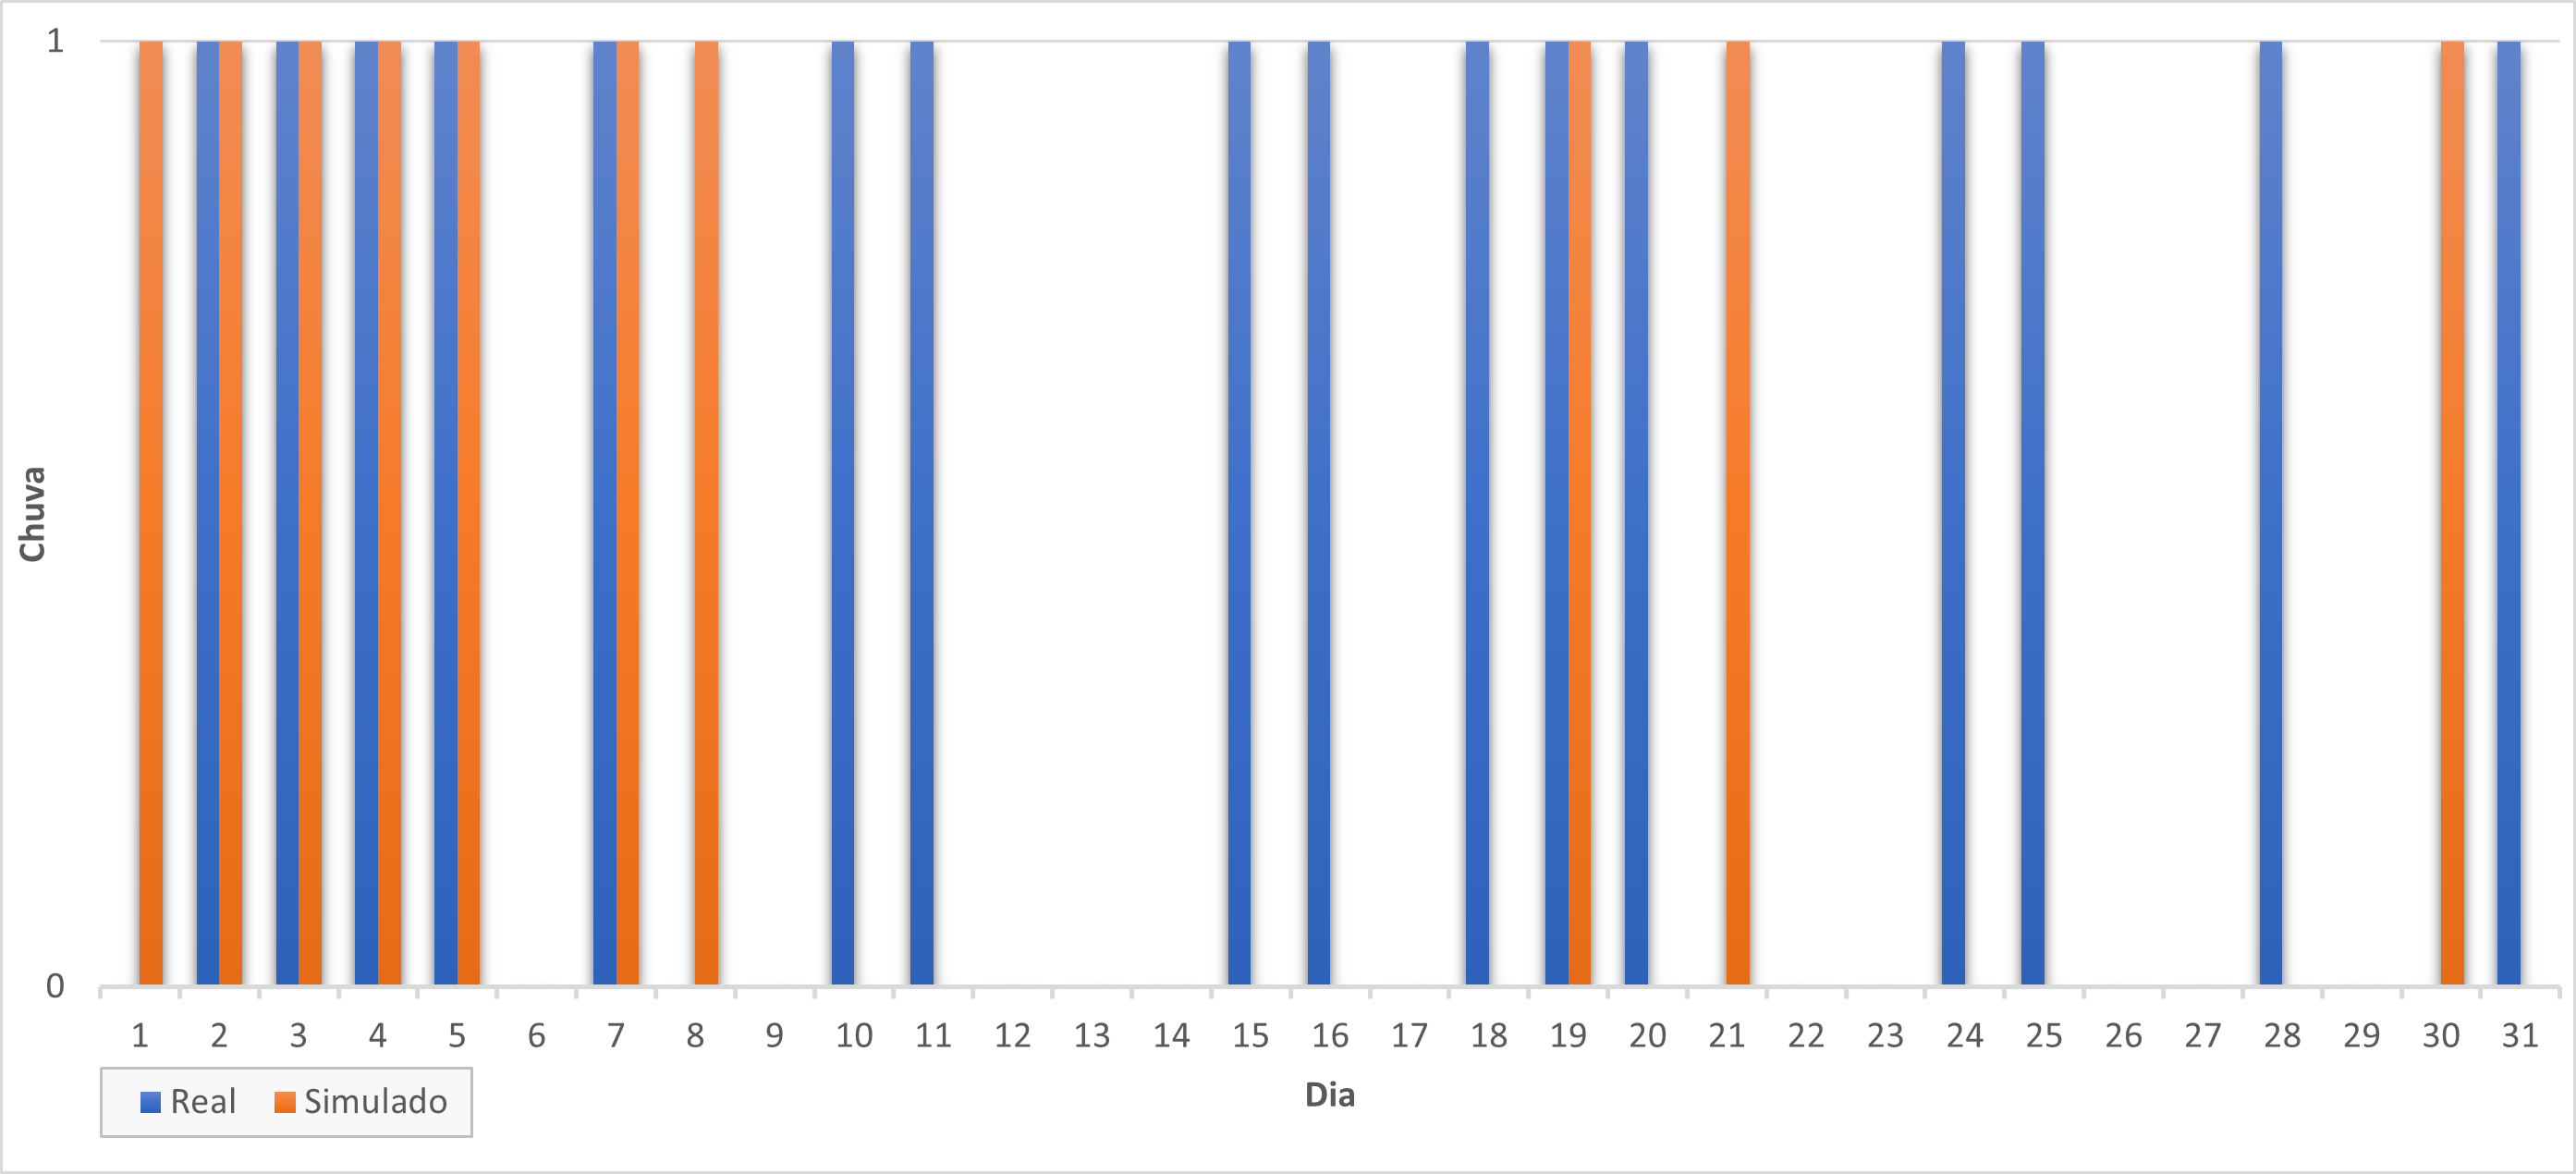
\includegraphics[width=\textwidth]{figs/out.png}
	\label{f.rout}
	\legend{\small Fonte: Elaborado pelo autor.}
\end{figure}

\subsection{Novembro}
Em novembro, 8 dias foram chuvosos e 22 foram secos. A simulação previu que 9 dias seriam chuvosos, porem não acertou corretamente as datas exatas de chuva no mês. Portanto, conforme mostrado na figura \ref{f.rnov}, apenas 43,33\% dos dias foram previstos corretamente.
\begin{figure}[H]
	\caption{\small Chuva x Dia - Novembro/2021}
	\centering
	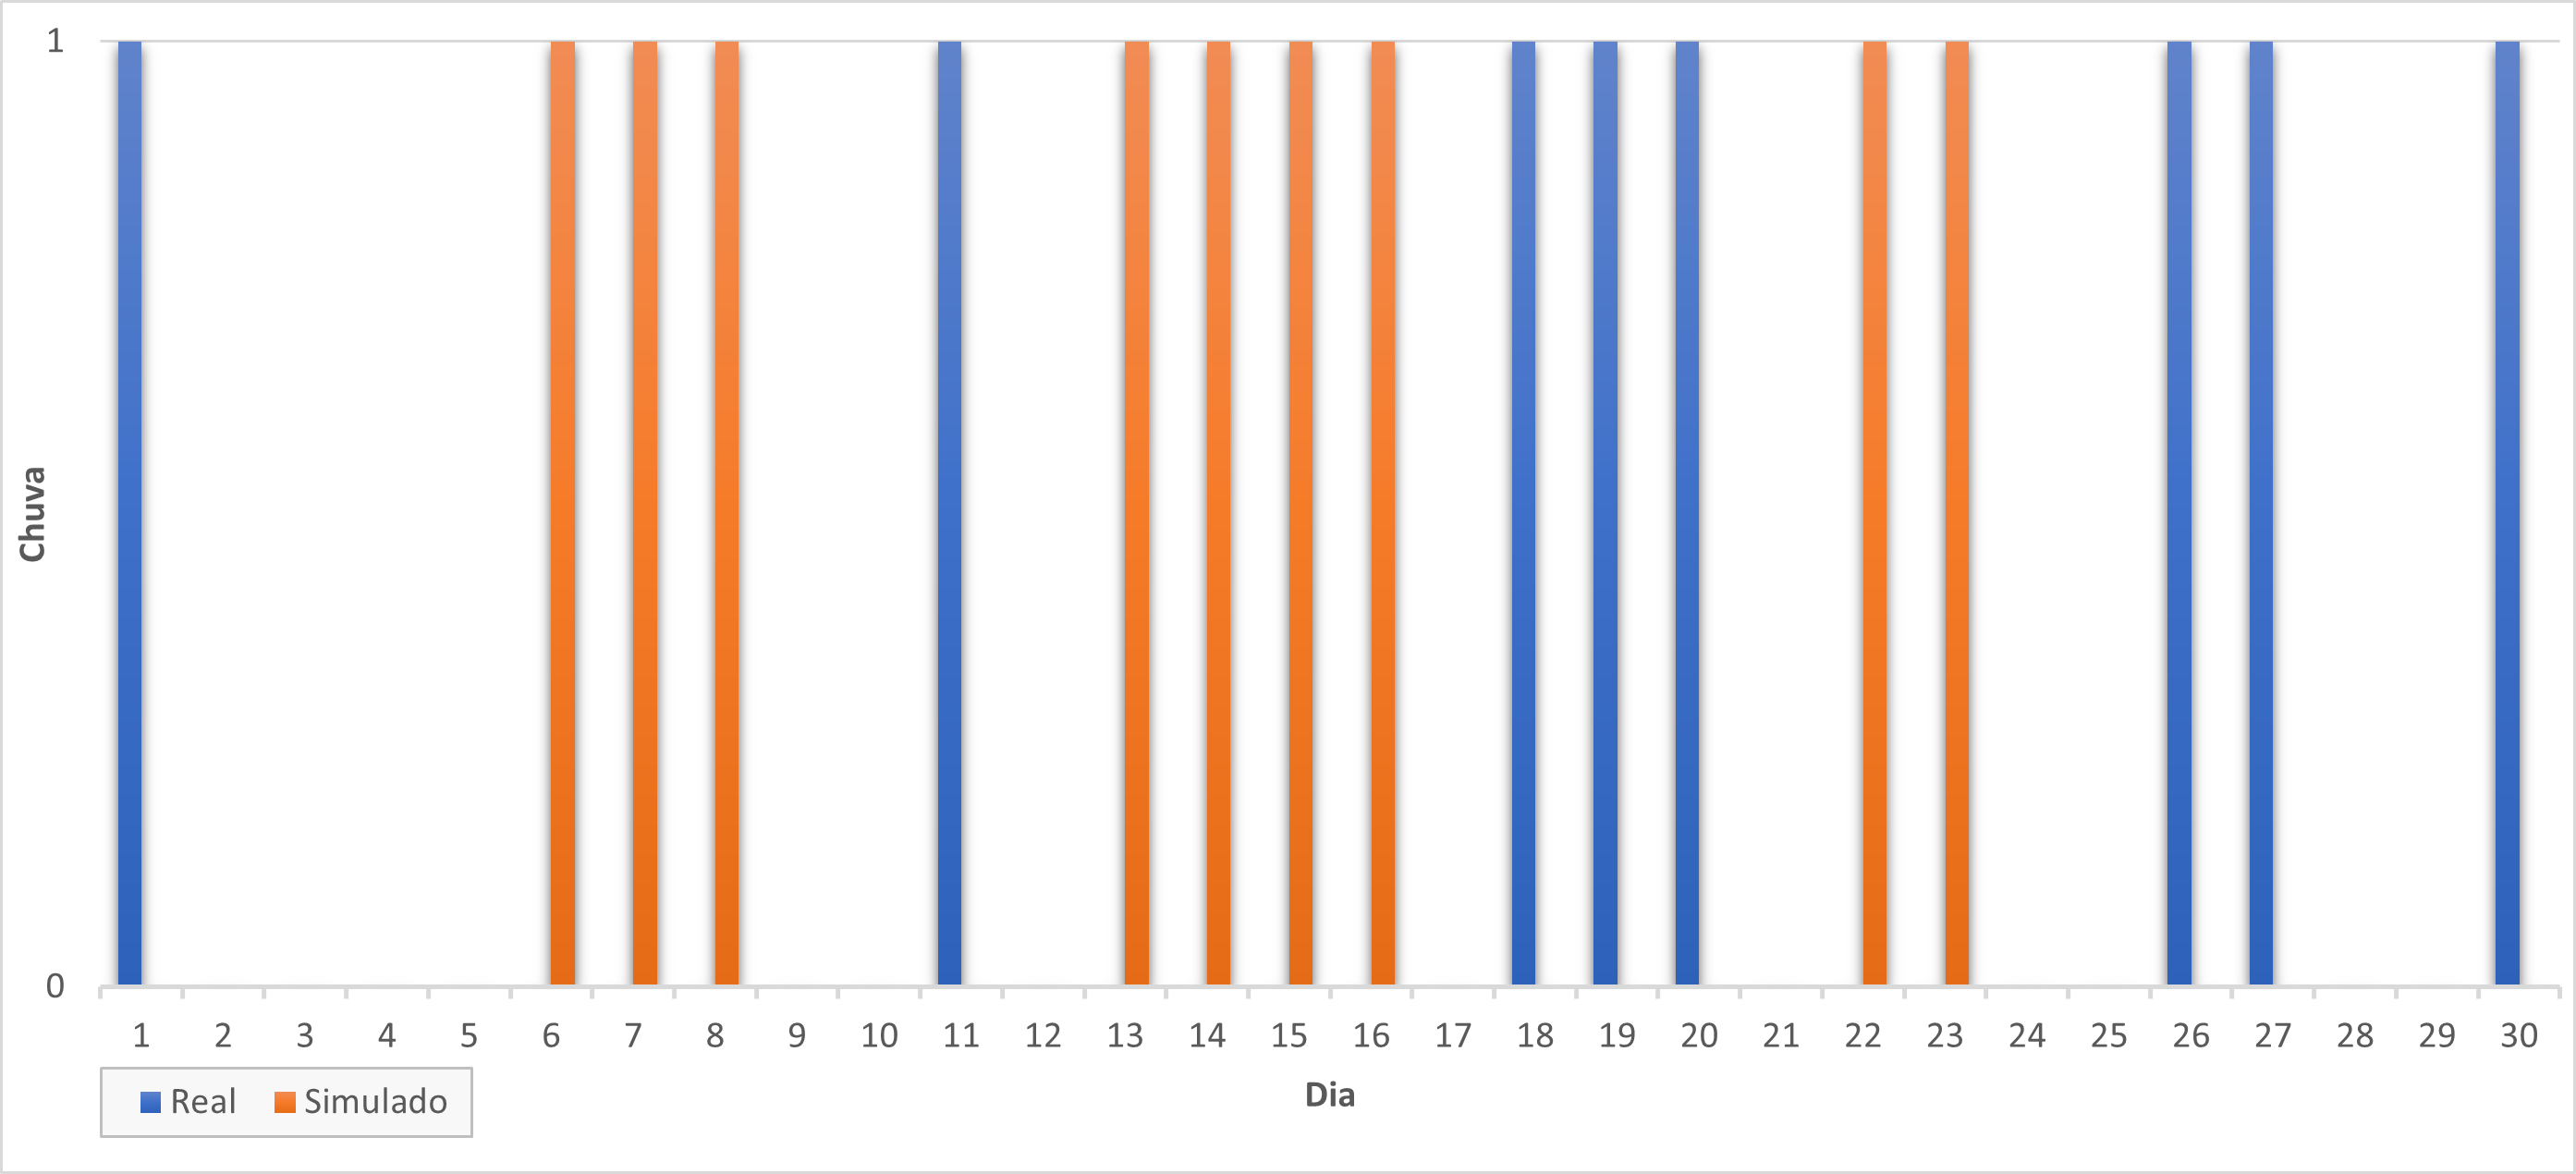
\includegraphics[width=\textwidth]{figs/nov.png}
	\label{f.rnov}
	\legend{\small Fonte: Elaborado pelo autor.}
\end{figure}

\subsection{Dezembro}
O último mês do ano geralmente é bastante chuvoso na cidade analisada. Em 2021, ano em que a simulação foi processada, foram 12 dias chuvosos. Muitos dos dias chuvosos foram previstos corretamente, assim como alguns dias secos, o que resultou em uma precisão de 58,06\% durante os 31 dias de dezembro.
\begin{figure}[H]
	\caption{\small Chuva x Dia - Dezembro/2021}
	\centering
	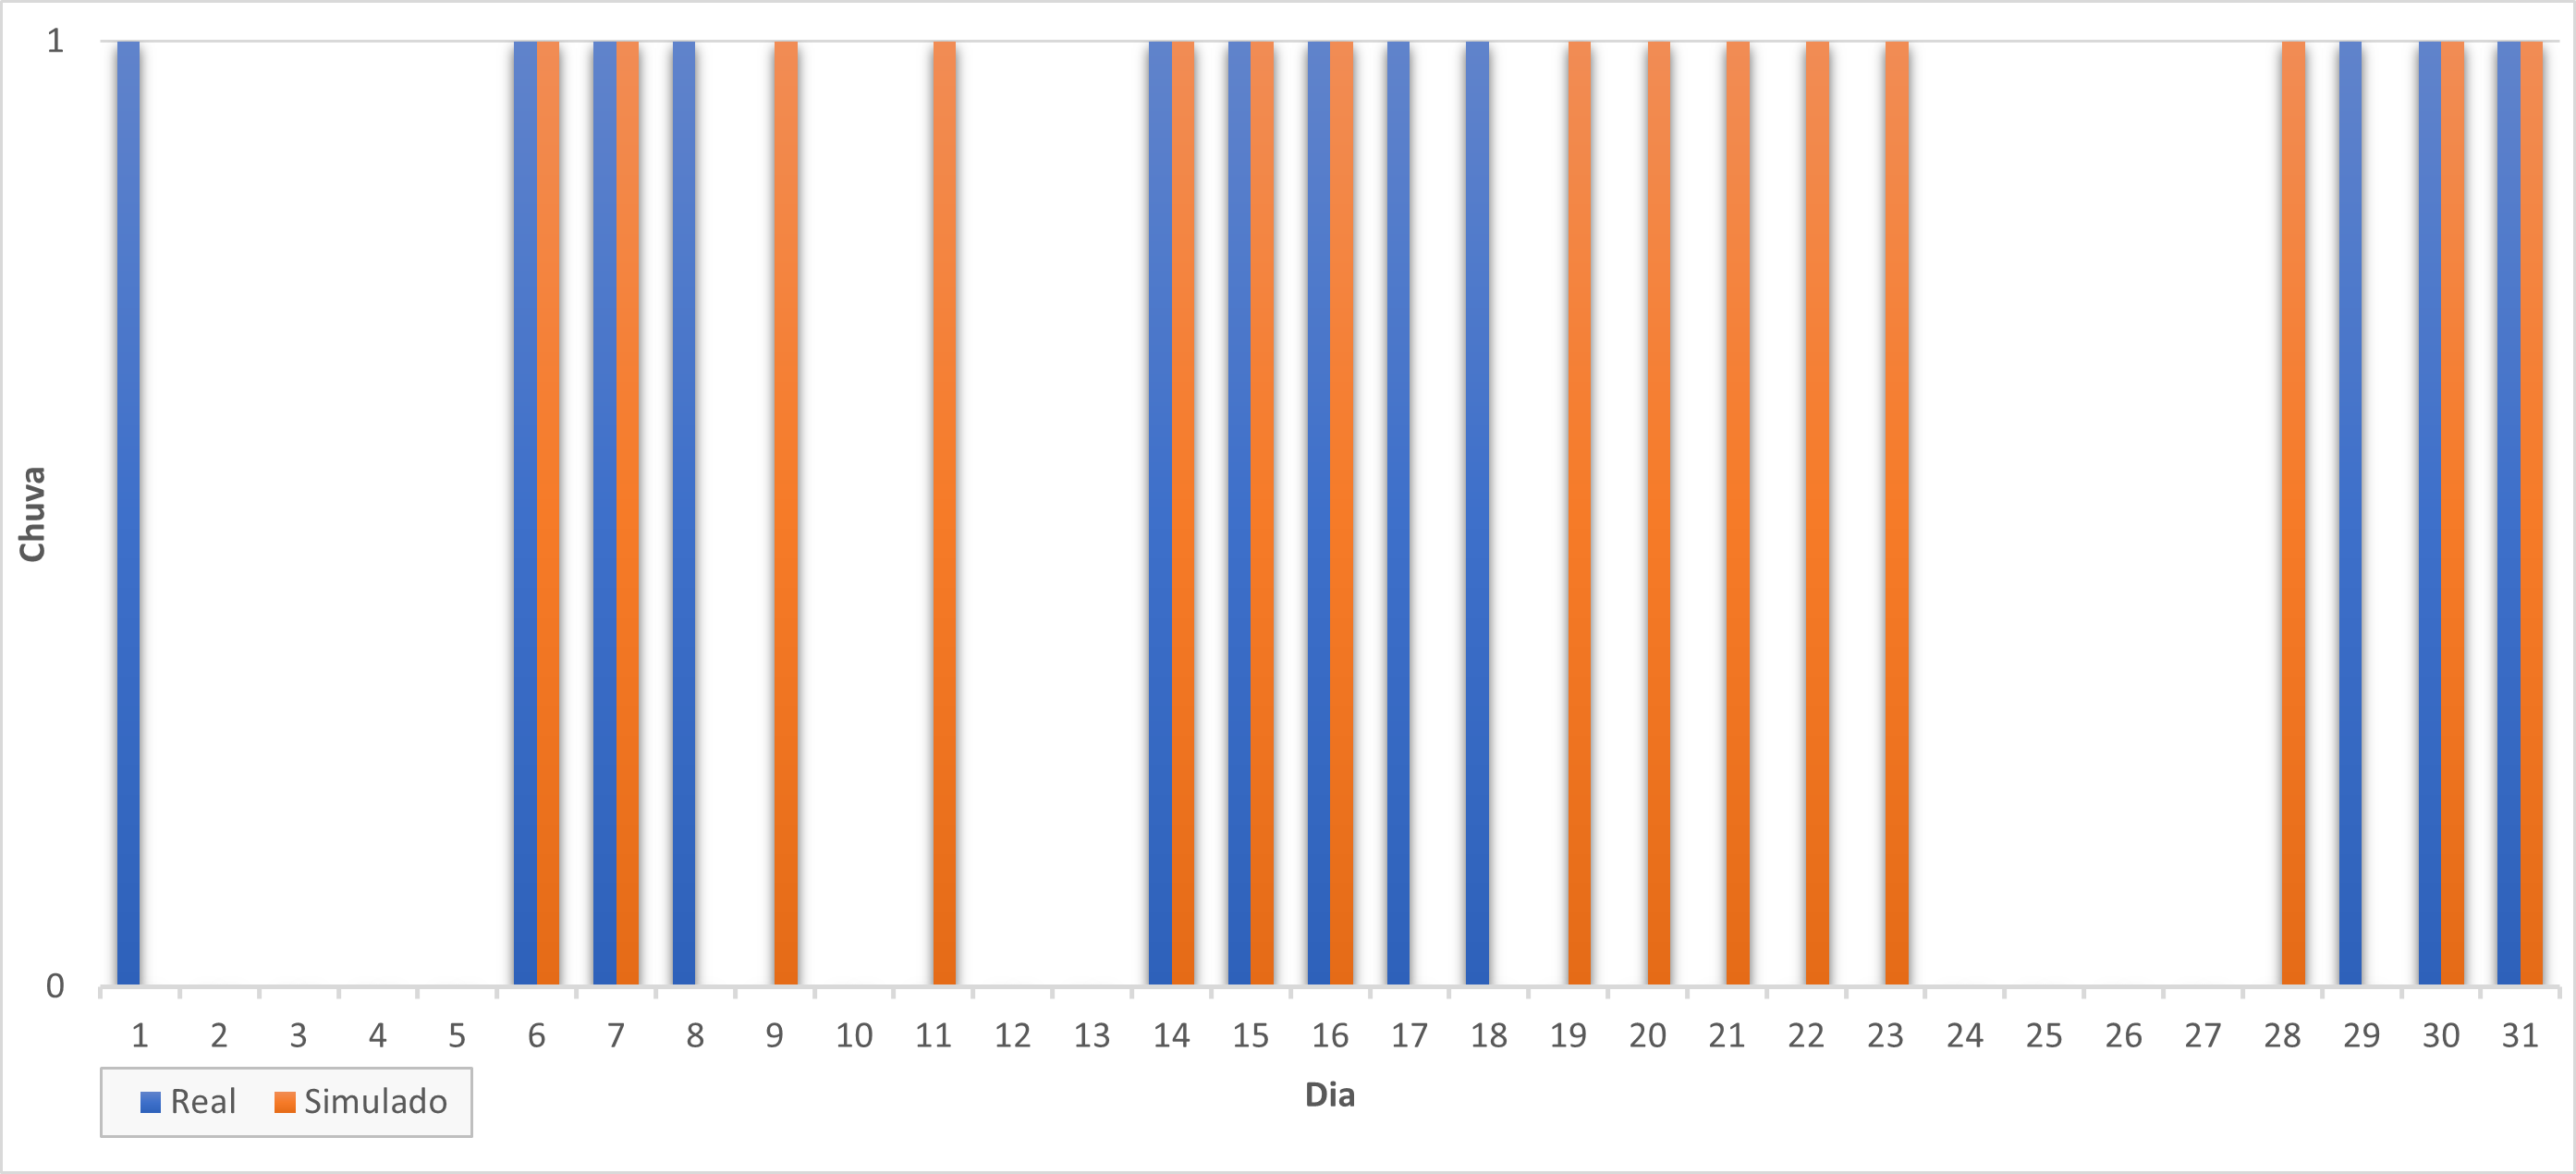
\includegraphics[width=\textwidth]{figs/dez.png}
	\label{f.rdez}
	\legend{\small Fonte: Elaborado pelo autor.}
\end{figure}


\section{Análise do ano}
Ao analisar o ano como um todo, o resultado teve alguns dados curiosos. A porcentagem de acerto média foi de 67\%, com um desvio padrão de 16,95 e coeficiente de variação de 25,43.

O mês com menor precisão de acertos foi novembro, com apenas 43,33\% dos dias previstos corretamente. Em julho e agosto, por serem meses muito secos, a simulação teve um desempenho maior, com 93,55\% de acerto.

Observando os 365 dias do ano de 2021 na cidade de Bauru, a partir dos dados do INMET, 98 dias tiveram precipitação maior do que 0mm \cite{inmet}, e foram considerados como dias chuvosos por este trabalho. Pela simulação computacional realizada, 101 dias foram previstos como chuvosos, um número muito próximo aos dados reais.